%% History:
% Pavel Tvrdik (26.12.2004)
%  + initial version for PhD Report
%
% Daniel Sykora (27.01.2005)
%
% Michal Valenta (3.12.2008)
% rada zmen ve formatovani (diky M. Duškovi, J. Holubovi a J. Žďárkovi)
% sjednoceni zdrojoveho kodu pro anglickou, ceskou, bakalarskou a diplomovou praci

% One-page layout: (proof-)reading on display
%%%% \documentclass[11pt,oneside,a4paper]{book}
% Two-page layout: final printing
\documentclass[11pt,twoside,a4paper]{book}   
%=-=-=-=-=-=-=-=-=-=-=-=--=%
% The user of this template may find useful to have an alternative to these 
% officially suggested packages:
\usepackage[czech, english]{babel}

\usepackage[T1]{fontenc} % pouzije EC fonty 
% pripadne pisete-li cesky, pak lze zkusit take:
% \usepackage[OT1]{fontenc} 
\usepackage[utf8]{inputenc}
%For code
\usepackage{listings}
\usepackage{upquote}
\lstset{
%language=JAVA,
%columns=fullflexible,
%showstringspaces=false
%frame=tb
language=JAVA,
basicstyle=\small\sffamily,
frame=tb,
columns=fullflexible,
showstringspaces=false
}
%=-=-=-=-=-=-=-=-=-=-=-=--=%
% In case of problems with PDF fonts, one may try to uncomment this line:
%\usepackage{lmodern}
%=-=-=-=-=-=-=-=-=-=-=-=--=%
%=-=-=-=-=-=-=-=-=-=-=-=--=%
% Depending on your particular TeX distribution and version of conversion tools 
% (dvips/dvipdf/ps2pdf), some (advanced | desperate) users may prefer to use 
% different settings.
% Please uncomment the following style and use your CSLaTeX (cslatex/pdfcslatex) 
% to process your work. Note however, this file is in UTF-8 and a conversion to 
% your native encoding may be required. Some settings below depend on babel 
% macros and should also be modified. See \selectlanguage \iflanguage.
%\usepackage{czech}  %%%%%\usepackage[T1]{czech} %%%%[IL2] [T1] [OT1]
%=-=-=-=-=-=-=-=-=-=-=-=--=%

%%%%%%%%%%%%%%%%%%%%%%%%%%%%%%%%%%%%%%%
% Styles required in your work follow %
%%%%%%%%%%%%%%%%%%%%%%%%%%%%%%%%%%%%%%%
\usepackage{graphicx}
%\usepackage{indentfirst} %1. odstavec jako v cestine.

\usepackage{k336_thesis_macros} % specialni makra pro formatovani DP a BP
 % muzete si vytvorit i sva vlastni v souboru k336_thesis_macros.sty
 % najdete  radu jednoduchych definic, ktere zde ani nejsou pouzity
 % napriklad: 
 % \newcommand{\bfig}{\begin{figure}\begin{center}}
 % \newcommand{\efig}{\end{center}\end{figure}}
 % umoznuje pouzit prikaz \bfig namisto \begin{figure}\begin{center} atd.


%%%%%%%%%%%%%%%%%%%%%%%%%%%%%%%%%%%%%
% Zvolte jednu z moznosti 
% Choose one of the following options
%%%%%%%%%%%%%%%%%%%%%%%%%%%%%%%%%%%%%
\newcommand\TypeOfWork{Diplomová práce} \typeout{Diplomova prace}
% \newcommand\TypeOfWork{Master's Thesis}   \typeout{Master's Thesis} 
%\newcommand\TypeOfWork{Bakalářská práce}  \typeout{Bakalarska prace}
% \newcommand\TypeOfWork{Bachelor's Project}  \typeout{Bachelor's Project}


%%%%%%%%%%%%%%%%%%%%%%%%%%%%%%%%%%%%%
% Zvolte jednu z moznosti 
% Choose one of the following options
%%%%%%%%%%%%%%%%%%%%%%%%%%%%%%%%%%%%%
% nabidky jsou z: http://www.fel.cvut.cz/cz/education/bk/prehled.html

%\newcommand\StudProgram{Elektrotechnika a informatika, dobíhající, Bakalářský}
%\newcommand\StudProgram{Elektrotechnika a informatika, dobíhající, Magisterský}
 %\newcommand\StudProgram{Elektrotechnika a informatika, strukturovaný, Bakalářský}
% \newcommand\StudProgram{Elektrotechnika a informatika, strukturovaný, Navazující magisterský}
\newcommand\StudProgram{Otevřená informatika, Magisterský}
% English study:
% \newcommand\StudProgram{Electrical Engineering and Information Technology}  % bachelor programe
% \newcommand\StudProgram{Electrical Engineering and Information Technology}  %master program


%%%%%%%%%%%%%%%%%%%%%%%%%%%%%%%%%%%%%
% Zvolte jednu z moznosti 
% Choose one of the following options
%%%%%%%%%%%%%%%%%%%%%%%%%%%%%%%%%%%%%
% nabidky jsou z: http://www.fel.cvut.cz/cz/education/bk/prehled.html

%\newcommand\StudBranch{Výpočetní technika}   % pro program EaI bak. (dobihajici i strukt.)
%\newcommand\StudBranch{Výpočetní technika}   % pro prgoram EaI mag. (dobihajici i strukt.)
\newcommand\StudBranch{Softwarové inženýrství}            %pro STM
%\newcommand\StudBranch{Web a multimedia}                  % pro STM
%\newcommand\StudBranch{Computer Engineering}              % bachelor programe
%\newcommand\StudBranch{Computer Science and Engineering}  % master programe


%%%%%%%%%%%%%%%%%%%%%%%%%%%%%%%%%%%%%%%%%%%%
% Vyplnte nazev prace, autora a vedouciho
% Set up Work Title, Author and Supervisor
%%%%%%%%%%%%%%%%%%%%%%%%%%%%%%%%%%%%%%%%%%%%

\newcommand\WorkTitle{ Aspektově orientovaný vývoj uživatelských rozhraní pro Java SE aplikace}
\newcommand\FirstandFamilyName{Bc. Martin Tomášek}
\newcommand\Supervisor{Ing. Tomáš Černý M.S.C.S. }


% Pouzijete-li pdflatex, tak je prijemne, kdyz bude mit vase prace
% funkcni odkazy i v pdf formatu
\usepackage[
pdftitle={\WorkTitle},
pdfauthor={\FirstandFamilyName},
bookmarks=true,
colorlinks=true,
breaklinks=true,
urlcolor=red,
citecolor=blue,
linkcolor=blue,
unicode=true,
]
{hyperref}



% Extension posted by Petr Dlouhy in order for better sources reference (\cite{} command) especially in Czech.
% April 2010
% See comment over \thebibliography command for details.

\usepackage[square, numbers]{natbib}             % sazba pouzite literatury
%\usepackage{url}
%\DeclareUrlCommand\url{\def\UrlLeft{<}\def\UrlRight{>}\urlstyle{tt}}  %rm/sf/tt
%\renewcommand{\emph}[1]{\textsl{#1}}    % melo by byt kurziva nebo sklonene,
\let\oldUrl\url
\renewcommand\url[1]{<\texttt{\oldUrl{#1}}>}




\begin{document}

%%%%%%%%%%%%%%%%%%%%%%%%%%%%%%%%%%%%%
% Zvolte jednu z moznosti 
% Choose one of the following options
%%%%%%%%%%%%%%%%%%%%%%%%%%%%%%%%%%%%%
\selectlanguage{czech}
%\selectlanguage{english} 

% prikaz \typeout vypise vyse uvedena nastaveni v prikazovem okne
% pro pohodlne ladeni prace


\iflanguage{czech}{
	 \typeout{************************************************}
	 \typeout{Zvoleny jazyk: cestina}
	 \typeout{Typ prace: \TypeOfWork}
	 \typeout{Studijni program: \StudProgram}
	 \typeout{Obor: \StudBranch}
	 \typeout{Jmeno: \FirstandFamilyName}
	 \typeout{Nazev prace: \WorkTitle}
	 \typeout{Vedouci prace: \Supervisor}
	 \typeout{***************************************************}
	 \newcommand\Department{Katedra počítačů}
	 \newcommand\Faculty{Fakulta elektrotechnická}
	 \newcommand\University{České vysoké učení technické v Praze}
	 \newcommand\labelSupervisor{Vedoucí práce}
	 \newcommand\labelStudProgram{Studijní program}
	 \newcommand\labelStudBranch{Obor}
}{
	 \typeout{************************************************}
	 \typeout{Language: english}
	 \typeout{Type of Work: \TypeOfWork}
	 \typeout{Study Program: \StudProgram}
	 \typeout{Study Branch: \StudBranch}
	 \typeout{Author: \FirstandFamilyName}
	 \typeout{Title: \WorkTitle}
	 \typeout{Supervisor: \Supervisor}
	 \typeout{***************************************************}
	 \newcommand\Department{Department of Computer Science and Engineering}
	 \newcommand\Faculty{Faculty of Electrical Engineering}
	 \newcommand\University{Czech Technical University in Prague}
	 \newcommand\labelSupervisor{Supervisor}
	 \newcommand\labelStudProgram{Study Programme} 
	 \newcommand\labelStudBranch{Field of Study}
}




%%%%%%%%%%%%%%%%%%%%%%%%%%    Poznamky ke kompletaci prace
% Nasledujici pasaz uzavrenou v {} ve sve praci samozrejme 
% zakomentujte nebo odstrante. 
% Ve vysledne svazane praci bude nahrazena skutecnym 
% oficialnim zadanim vasi prace.

%%%%%%%%%%%%%%%%%%%%%%%%%%    Titulni stranka / Title page 

\coverpagestarts

%%%%%%%%%%%%%%%%%%%%%%%%%%%    Podekovani / Acknowledgements 

\acknowledgements
\noindent
Tímto bych rád poděkoval celé svojí rodině za podporu během studia. Dále bych rád poděkoval vedoucíme mé diplomové práce panu Ing. Tomáši Černému za ochotu, pomoc, čas, zkušenosti a příležitosti, které mi poskytoval během celého mého studia. 

%%%%%%%%%%%%%%%%%%%%%%%%%%%   Prohlaseni / Declaration 

\declaration{Ve~Strakonicích 17.\,5.\,2012}
%\declaration{In Kořenovice nad Bečvárkou on May 15, 2008}


%%%%%%%%%%%%%%%%%%%%%%%%%%%%    Abstract 
 
\abstractpage

In this modern and rush age there is expected that every employee will create their task and refer outputs. Entering these tasks and their record is time, money and effort consuming. Information systems are nowadays integral part of organization structure and they make work easier to all people who use them. These systems are known as e-learning systems in university campus. This bachelor thesis is focused on  development of the information system in Java language, which facilitate task entering, managing and submissioning. In the first part is introduced the design of the system and in the second part is introduced the implementation and testing of the software.

% Prace v cestine musi krome abstraktu v anglictine obsahovat i
% abstrakt v cestine.
\vglue60mm

\noindent{\Huge \textbf{Abstrakt}}
\vskip 2.75\baselineskip

\noindent
V dnešní moderní a uspěchané době se od každého zaměstnance očekává, že bude plnit zadané úkoly a odevzdávat výstupy z nich plynoucí. Zadávání těchto úloh a jejich evidence stojí určité množství času, peněz a úsilí. Informační systémy jsou dnes již nedílnou součástí organizační činnosti a usnadňují práci všem zainteresovaným osobám. Na akademické půdě jsou známy především jako e-learning systémy. Tato bakalářská práce se zaměřuje na návrh a vývoj informačního systému v jazyku Java, který usnadní zadávání, evidenci a odevzdávání úkolů. V první části je představen návrh systému a v druhé části je představena jeho implementace spolu s testováním.  

%%%%%%%%%%%%%%%%%%%%%%%%%%%%%%%%  Obsah / Table of Contents 

\tableofcontents


%%%%%%%%%%%%%%%%%%%%%%%%%%%%%%%  Seznam obrazku / List of Figures 

\listoffigures


%%%%%%%%%%%%%%%%%%%%%%%%%%%%%%%  Seznam tabulek / List of Tables

\listoftables
\renewcommand\lstlistingname{Část zdrojového kódu}
\renewcommand\lstlistlistingname{Seznam částí zdrojových kódů}
\lstlistoflistings


%**************************************************************

\mainbodystarts
% horizontalní mezera mezi dvema odstavci
%\parskip=5pt
%11.12.2008 parskip + tolerance
\normalfont
\parskip=0.2\baselineskip plus 0.2\baselineskip minus 0.1\baselineskip

% Odsazeni prvniho radku odstavce resi class book (neaplikuje se na prvni 
% odstavce kapitol, sekci, podsekci atd.) Viz usepackage{indentfirst}.
% Chcete-li selektivne zamezit odsazeni 1. radku nektereho odstavce,
% pouzijte prikaz \noindent.

%**************************************************************

% Pro snadnejsi praci s vetsimi texty je rozumne tyto rozdelit
% do samostatnych souboru nejlepe dle kapitol a tyto potom vkladat
% pomoci prikazu \include{jmeno_souboru.tex} nebo \include{jmeno_souboru}.
% Napr.:
% \chapter{Úvod}
Tato bakalářská práce se zabývá analýzou, návrhem a otestováním frameworků pro mobilní platformy Android a Windows Phone. Tyto frameworky interpretují uživatelské rozhraní z dat generovaných serverem z modelu, která jsou poskytována serverem pomocí webových služeb.

První část práce popisuje aktuální situaci v tvorbě UI, specifikuje požadavky a cíle práce a zkoumá již existující řešení. V druhé části se analyzují požadavky, které by měla práce splňovat, a návrh řešení, které stanovené požadavky a cíle splňuje. Ve třetí části je popsána struktura a vlastní implementace řešení. Poslední část obsahuje otestování řešení a ukazuje vzorové aplikace na dvou různých mobilních prostředích.

Práce obsahuje seznam použitých zkratek, které lze nalézt v příloze A, instalační příručku v příloze B, použité UML diagramy a obrázky viz příloha C, ukázky zdrojových kódů v příloze D a obsah CD s prací a zdrojovými kódy je v příloze E.
 
\section{Motivace}
Nedílnou součástí většiny dnešních aplikací je uživatelské rozhraní. Uživatelské rozhraní by mělo uživateli co nejvíce usnadňovat manipulaci se softwarem a tudíž být intuitivní a použitelné, mělo by mít adekvátní design, nejlépe korespondující s aktuálními trendy. Vývoj takového rozhraní je však časově velmi náročný proces, který zahrnuje nejenom samotný vývoj, ale také rozsáhlé testování, hlavně z hlediska funkčnosti a použitelnosti. Celý problém navíc umocňuje fakt, že se vývojáři snaží zajistit podporu softwaru na více platformách, neboť chtějí uživatelům nabídnout možnost operovat s jejich vytvořeným systémem nejen z počítače či laptopu, ale také z tabletu nebo mobilního zařízení. Mobilní verze grafického uživatelského rozhraní nebývá často moc rozdílná od rozhraní ostatních platforem v tom smyslu, že se v ní vyskytují převážně stejné grafické prvky, a tak pro mobilní verzi vzniká téměř indentická kopie tohoto rozhraní, což vede i k duplicitě v kódu aplikace \cite{on-web-services}. Problémem je, že se často uživatelská rozhraní mění, ať už se změna týká rozložení komponent, přidání nebo odebrání komponenty nebo třeba validace uživatelského vstupu, protože takováto změna se musí provést na všech platformách a někdy i na více místech v rámci aplikace, což může být v případě rozsáhlých systémů nejednoduchý úkol, který stojí vývojáře spoustu zbytečného času a může vést i ke vzniku nových typů chyb \cite{towards-smart-design}. Pokud bychom byli schopni nadefinovat uživatelské rozhraní jen jednou pro všechny platformy na jednom místě, tento problém bychom odstranili. Definice by tedy byla obecná, ale každá platforma je jiná a něčím specifická, proto je třeba vytvořit pro různé platformy frameworky, které obecnou definici pro danou platformu interpretují. 

Bylo mi nabítnuto vytvořit takovýto framework pro dvě mobilní platformy, kontrétně pro Android a Windows Phone, což mi přislo velmi užitečné a zajímavé, a proto jsem se rozhodl zpracovat toto téma jako bakalářskou práci.

% \include{2_teorie}
% atd...

%*****************************************************************************
\chapter{Úvod}
Tato bakalářská práce se zabývá analýzou, návrhem a otestováním frameworků pro mobilní platformy Android a Windows Phone. Tyto frameworky interpretují uživatelské rozhraní z dat generovaných serverem z modelu, která jsou poskytována serverem pomocí webových služeb.

První část práce popisuje aktuální situaci v tvorbě UI, specifikuje požadavky a cíle práce a zkoumá již existující řešení. V druhé části se analyzují požadavky, které by měla práce splňovat, a návrh řešení, které stanovené požadavky a cíle splňuje. Ve třetí části je popsána struktura a vlastní implementace řešení. Poslední část obsahuje otestování řešení a ukazuje vzorové aplikace na dvou různých mobilních prostředích.

Práce obsahuje seznam použitých zkratek, které lze nalézt v příloze A, instalační příručku v příloze B, použité UML diagramy a obrázky viz příloha C, ukázky zdrojových kódů v příloze D a obsah CD s prací a zdrojovými kódy je v příloze E.
 
\section{Motivace}
Nedílnou součástí většiny dnešních aplikací je uživatelské rozhraní. Uživatelské rozhraní by mělo uživateli co nejvíce usnadňovat manipulaci se softwarem a tudíž být intuitivní a použitelné, mělo by mít adekvátní design, nejlépe korespondující s aktuálními trendy. Vývoj takového rozhraní je však časově velmi náročný proces, který zahrnuje nejenom samotný vývoj, ale také rozsáhlé testování, hlavně z hlediska funkčnosti a použitelnosti. Celý problém navíc umocňuje fakt, že se vývojáři snaží zajistit podporu softwaru na více platformách, neboť chtějí uživatelům nabídnout možnost operovat s jejich vytvořeným systémem nejen z počítače či laptopu, ale také z tabletu nebo mobilního zařízení. Mobilní verze grafického uživatelského rozhraní nebývá často moc rozdílná od rozhraní ostatních platforem v tom smyslu, že se v ní vyskytují převážně stejné grafické prvky, a tak pro mobilní verzi vzniká téměř indentická kopie tohoto rozhraní, což vede i k duplicitě v kódu aplikace \cite{on-web-services}. Problémem je, že se často uživatelská rozhraní mění, ať už se změna týká rozložení komponent, přidání nebo odebrání komponenty nebo třeba validace uživatelského vstupu, protože takováto změna se musí provést na všech platformách a někdy i na více místech v rámci aplikace, což může být v případě rozsáhlých systémů nejednoduchý úkol, který stojí vývojáře spoustu zbytečného času a může vést i ke vzniku nových typů chyb \cite{towards-smart-design}. Pokud bychom byli schopni nadefinovat uživatelské rozhraní jen jednou pro všechny platformy na jednom místě, tento problém bychom odstranili. Definice by tedy byla obecná, ale každá platforma je jiná a něčím specifická, proto je třeba vytvořit pro různé platformy frameworky, které obecnou definici pro danou platformu interpretují. 

Bylo mi nabítnuto vytvořit takovýto framework pro dvě mobilní platformy, kontrétně pro Android a Windows Phone, což mi přislo velmi užitečné a zajímavé, a proto jsem se rozhodl zpracovat toto téma jako bakalářskou práci.

\chapter{Popis problému a specifikace cíle}
\section{Popis problematiky}
Softwarové systémy jsou určeny k tomu, aby méně či více úspěšně poskytovali uživateli nástroj, který mu pomůže s řešením problémů. Systém tedy musí komunikovat s uživatelem. K tomuto účelu se využívá uživatelské rozhraní. Vývoj uživatelského rozhraní zabere přibližně 50 \% času \cite{cernyTSUID}, který je určen na vývoj konkrétního systému. Tento údaj se samozřejmě může lišit v závislosti na účelu a velikosti systému. Při tvorbě uživatelského rozhraní se obvykle zaměřujeme na použitelnost. V tomto případě provádíme testy použitelnosti na cílové skupině, na jejichž základě jsme schopni určit, zdali je návrh použitelný či nikoliv. Důvodem tohoto testování je fakt, že obvykle systém vyvtváříme pro uživatele a ne obráceně. Z výše uvedených skutečností vyplívá, že je potřeba uživatelské rozhraní důkladně testovat, aby bylo pro cílovou skupinu správně použitelné. Bohužel, když se hovoří o uživatelském rozhraní, tak se často zapomíná na to, že toto rozhraní se musí nejen vytvořit, ale také udržovat. Softwarový systém tráví většinu svého života v udržovacím režimu, kterému se říká support nebo li podpora. V této fázi přichází na systém mnoho požadavků, které musí být proveditelné a to za přijatelné náklady. Nedílnou součástí jsou změny, které se týkají databázového modelu a obvykle tyto změny musí reflektovat UI. Podívejme se proto na systém z pohledu vývojáře. Systém pro něj musí být snadno udržovatelný, změny lehce proveditelné a bez větších dopadů na systém. V tomto případě by bylo vhodné reflektovat tyto změny v UI. Nedílnou součástí každého uživatelského rozhraní jsou validace, které by měli reflektovat například změny v databázovém modelu ale i změny v business modelu.
\subsection{Typy uživatelských rozhraní}
Jak již bylo zmíněno, tak uživatelské rozhraní se testuje na základě typu aplikace a jejím použití. Je také důležité vzít v potaz zařízení, na kterém je aplikace provozována. Může se jednat o desktopovou, mobilní či serverou aplikaci. V každém z výše uvedených případů bude návrh uživatelského rohraní podíměn jinými faktory, které jsou specifické pro dané zařízení. Těmito faktory jsou způsoby, jakými se aplikace ovládá, prostředí, v kterém se uživatel právě nachází a účel, ke kterému je aplikace určena. Například aplikace na mobilních zařízení nemusí podporovat klávesové zkratky, ale mohla by podporovat gesta. Obdobně aplikace použitá na desktopu může počítat s použití myše, touchpadu, klávesnice - jak standardní tak dotykové, či jiného externího zařízení. Je tedy zřejmé, že uživatelské rozhraní je kromě jeho účelu podmíněno i zařízením, na kterém je používáno.

Základnímy ovládacími a vizuálními prvky téměř každé aplikace prvky jsou tlačítka, vstupní pole, přepínače, tabulky, menu a statické texty. Vstupní pole můžeme shrnout do jedné kategorie, která se nazývá formulář. Formulář obvykle osahuje 1 až N prvků, s tím, že každý prvek má zde svojí funkčnost a účel. Účelem je poskytnout uživateli možnost vložení dat, či možnost volby chování aplikace. Funkčností je tato data správně interpretovat a na jejich základě provést specifické akce. Ve formuláři také mohou být pouze statická data, která slouží k reprezentaci aktuálního stavu, který slouží uživateli k tomu, aby pochopil aktuální stav ve kterém se aplikace či jeho část nachází a na základě tohoto stavu mohl rozhodnout o další akci, pokud je toto rozhodnutí vyžadování a umožněno.
\subsection{Získávání a vkládání dat}
Aplikace použí vizuální prvky k tomu, aby uživateli reprezentovala data či umožňila uživateli tato data vytvořit. Moderním způsobem je dnes využívat k získávání a vkládání dat webové služby. Výhodou je, že se klient může připojit na různé zdroje a z těchto dat si vytvářet tzv: mashup. Obvyklé použití je takové, že server získá data z více zdrojů a ty pak interpretuje klientům. Klient tedy nezná orignální původ informací. Jedním z dalších způsobů je vlastní databáze na klientovi. V tomto případě již ale nemůžeme hovořit o klientovi, neboť se jedná o soběstačnou aplikaci, v případě, že nezískává data z jiných dalších zdrojů. Samozřejmě existují i kombinace těchto možností. Volba závisí vždy na konkrétním zadání a účelu, pro který je aplikace navržena.

V případě reprezentace je potřeba data získat. Jak již zbylo zmíněno výše existuje mnoho způsobů kde a jak data získat. Zaměříme se nyní na získání dat z jiných zdrojů. Pokud žádáme o data jiný zdroj, tak jsme obvykle schopni zjistit formát a způsob, jakým o data požádat, ale formát dat neznáme. Nejčastěji jsou data přenásena jako JSON \cite{javaEE} nebo XML. To nám umožní data serializovat do objektu, pokud známe definici objektu. Definice objektu lze získat obvykle v dokumentaci k dané službě, takže námi navržená aplikace očekává data specifického typu. Uvažujme nyní příklad, kdy jsme vytvořili klienta, který zobrazuje jména a příjmení uživatelů v systému. Po určité době, je však potřeba kromě jména i zobrazovat jejich uživatelské jméno. Do dat, která získáváme od služby tedy přibude sloupeček s uživatelským jménem. Nyní musíme naší klientskou aplikaci upravit, tak aby byla schopná zobrazovat i tyto informace. Provedli jsme tady poměrně triviální úpravu. Přidali jsme pole k zobrazení uživatelského jména, upravili jsme objekt, do kterého se data serializovala a v další verzi vydání aplikace se tato změna projeví. Změna tedy není klientům dostupná ihned. Po uričté době se rozhodlo, že se kolonka uživatelského jména odstraní. Tento případ je tedy mnohem horší. Neboť po serializace bude v poli reprezentující uživatelské jméno hodnota null. Pokud jsme jméno pouze vypisovali tak je vše v pořádku, avašak pokud jsme nad ním volali nějaké operace můžeme obdržet vyjímku a aplikace nebude schopna pokračovat v běhu.

V případě vkládání dat do jiného zdroje platí chování a nastavení z odstavce uvedeného výše. Je tedy potřeba znát zdroj, na který data odeslat, formát dat, metodu a popřípadě další dodatečná nastavení služby. Budeme uvažovat stejný příklad jako byl již rozebrán v předchozím odstavci s tím rozdílem, že nyní data vkládáme. Na server tedy nejprve odesíláme pouze jméno a přijímení. Předpokládejme, že tyto dvě hodny jsou serverem vyžadovány. Je tedy potřeba mít validaci, která hlídá zdali jsou data před odesláním v pořádku, či správně interpretovat odpověď serveru, který sdělí, že data nejsou validní, pokud touto validací disponuje. Při přidání nového pole, u kterého server vyžaduje jeho vyplnění nyní klient přestane správně fungovat a server by měl data odmítat. Musíme tedy udělat změnu na klientovi. Přidat vstupní pole, přidat proměnou, která bude zastupovat uživatelské jméno a novou verzi nasadit a distribuovat. Po určité době, stejně jako v prvním případě se definice dat změní a uživatelské jméno již nebude klientům zasíláno a nebude ani možnost ho vyplňovat. Klient se opět stane nevalidním, neboť při serializaci na straně serveru dojde k chybě, protože klient posílá proměnou, kterou již nyní server neznám. Formulář se tedy opět stane nefunkčním.
 
\subsection{Aspektový přístup}
Z dosavadního testu je zřejmé, že aplikace obsahuje vizuální prvky, na které lze nahlížet z několika aspektů. Jedním z důležitých aspektů je bezpečnost. Funkce, které může konkrétní uživatel využívat se přidělují na základě uživatelských rolí. V této souvislosti je mnoho přístupů jak role přidělovat a spravovat, ale všechny způsoby mají jedno společné. Ověřeřují, zdali má uživatel právo akci provádět. Souvislost mezi rolí a uživatelským rozhraním je patrá. Mějmě uživatele v role administrátora. Tato role bude mít práva na úpravu uživatelských dat jiných uživatelů. Dále mějme roli hosta, která si může data uživatelů pouze zobrazit. Při detailnějším prozkoumání zjistíme, že existuje množina zobrazovaných dat, která je pro obě role stejná, nicméně pro roli hosta by měla být všechna tato data needitovatelná. Dosáhnout této možnosti lze několika způsoby a záleží na platformě a volbě řešení. Nicméně v Java SE aplikaci, která využívá SWING to znamená, že buď musí být data zobrazována jakou label nebo musí být komponenty vypnuty. V obou případech musí vývojář na základě uživatelské role zvolit jeden z přístupů a nastavovat data na konkrétní komponentě. Pokud zvolí způsob labelů, tak vytváří duplicitní formulář pouze s jiným aktivním prvkem. Pokud jsou data získávána ze serveru, tak na něm jsou již bezpečnostní politiky implementované a postačilo by jejich výsledky propagovat do klientské aplikace. Server by tedy sám rozhodl, jaká data zobrazit.
\section{Existující řešení}
V současné době existuje několik řešení, které se snaží zjednodušit tvorbu uživatelského rozrahní. Níže zmíněné technologie se zaměřují pouze na konkrétní framework. Například JSF, JSP,  Swing, Android, Struts, Vaadin. Tyto řešení se zaměřují na inspekci objektů, která již nesou informace o daném objektu. Výhodou inspekce za běhu programu je to, že dokáží na základě typu dat postavit přesné uživatelské rozhraní. Mezi hlavní nevýhody patří samotné generování uživatelského rozhraní, které se dále velmi špatně donastavuje a samozřejmě také fakt, že pro inspekci je obvykle využita reflekce. Níže jsou uvedeny současné frameworky, které umožňují vytvářet generovaná uživatelská rozhraní.
\subsection{SwinXml}
Tento framework se zaměřuje pouze na generování uživatelského rozhraní ve Swingu. Základem je specifikace rozhraní pomocí XML, což je velmi velkou výhodou. neboť specifikace v tomot formátu má jasně dané možnosti a je na první pohled zřejmé jak bude dáná komponenta fungovat. Knihovna implementuje téměř všechny možnosti, které lze nastavit standardní cestou vývoje Swing aplikace. ActionListenery a dodatečné nastavení si vývojář může specifkovat po vygenerování komponent. Hlavní nevýhodou je, že všechny komponenty, které se generují je potřeba mít specifikované i ve výsledné aplikaci. Není zde žádné zapouzdření komponent a při detailnější specifikaci se stává XML definice až příliš rozsáhlá.
\subsection{Metawidget}
Projekt Metawidget se zaměřuje na vytváření uživateského rozhraní na základě inspekce tříd. Použít ji lze z mnoha populárními frameworky jako jsou Spring, Struts, JSF, JSP a další. Generování uživatelského rozhraní probíhá na základě inspekce již existující třídy a konfigurace konkrétní aplikace. Aktuální verze je 4.0 a vyšla 1.listopadu 2014. Jsou k dispozici pod licencí LGPL/EPL. Co se týče použitelnosti frameworku tak je Mezi hlavní výhody této knihovny patří zejména široká škála podporovaných frameworků a hlavně velká škála podporovaných validátorů. Data lze získat i pomocí REST, nicméně nativní a jednoduchá podpora zde chybí. Framework bohužel neumožňuje generování tabulek.
\subsection{AspectFaces}
Jedná se o framework, který umožňuje inspekci na základě tříd. Framework umožňuje použití různých layoutů a inspekčních pravidel. Výsledné vygenerované uživatelské rozhraní se může pro stejné obejkty lišit na základě specifického nastavení. V současné době je stabilní verze 1.4.0 a na verzi 1.5.0 se pracuje. Vývojář si může své vlastní nastavení generování tříd upravit. Tato nastavení jsou v XML formátu a lze je tedy snadno modifikovat. Framework podporuje velkou škálu anotací z JPA, Hibernate a uživatel si v případě nutnosti může vytvořit vlastní antoaci, která se promítne do inspekce. Framework je prozatím bohužel jednostranně orientovaný na JSF. Tomu odpovídá i způsob generování dat a způsob, jakým je prováděna složitější inspekce. 
\section{Cíle projektu}
Existující řešení poskytují mnoho různorodých funkcí. Jejich hlavními výhody jsou zkrácení času, který je potřeba k vývoji a úpravě uživatelského rozhraní. V trendem současné doby jsou webové služby, proto se i v této práci bude soustředit na získávání definice dat z webových služeb a jejích interpretaci na klienta stejně tak jako na plnění této reprezentace skutečnými daty. Inspekce tedy bude prováděna na straně serveru, který zná objekty, s kterými pracuje a klient pouze obdrží jejich definici. Tento přístup umožńí klientovi pružně a ihned reagovat na změny v datovém formátu, který diktuje server. Dalším pozitivním vlivem, bude to, že server bude klientovi poskytovat i seznam validací, jimiž musí jednotlivá komponenta vyhovět, aby bylo možné data odeslat zpět na server a ten je správně zpracoval. Celý tento proces by měl být pro kleinta zapouzdřen, aby aplikace nevyžadovala od klienta více informací než je nutné. Mezi nutnou informaci patří specifikace připojení a formát dat. Například JSON, XML. Použítí frameworku by mělo být velmi jednoduché a v případě, že bude chtít klient postavit formulář, tak by mu mělo stačit pouze několik řádků kódu. Dalším důležitým aspektem jsou již existující zdroje na serveru, které by měli po přidání frameworku zůstat stejné.   
 
\chapter{Analýza}
\section{Funkční specifikace}
Framework \cite{framework} musí uživateli umožňovat vytvářet a dále pracovat s vytvořenými komponentami. Komponenty budou procházet určitým životním cyklem. Kromě samotných komponent musí framework poskytovat i dodatečné funkcionality, které jsou spojeny se získáváním dat, jejich propagací na klienta, zabezpečení, organizací komponent, lokalizací a skinováním komponent.
\subsection{Funkční požadavky}
Z dosavadního popisu problému byly vytvořeny následující požadavky na systém.
\begin{itemize}
\item Framework bude umožňovat generovat metadata objektů, na základě kterých budou generovány komponenty.
\item Framework bude umožňovat vygenerovat formulář nebo tabulku na základě dat získaných ze serveru.
\item Framework bude generovat metadata, která nebudou závislá na platformě.
\item Framework bude umožňovat získat data ze serveru.
\item Framework bude umožňovat naplnit formulář i tabulku daty.
\item Framework bude umožňovat odeslat data z formuláře zpět na server.
\item Framework bude umožňovat používat lokalizační resource bundly.
\item Framework bude umožňovat validaci dat na základě metadat, která obdržel od serveru.
\item Framework bude umožňovat klientovi překrýt chybové validační hlášky.
\item Framework bude umožňovat skinovatelnost.
\item Framework bude umožňovat specifikovat zdroje ve formátu XML.
\item Framework bude umožňovat vytvářet vstupní pole, combo boxy, výstupní pole, textarea, checkboxy, option buttony.
\item Framework bude umožňovat vkládat do formulářových polí texty, čísla a datum.
\item Framework bude umožňovat generování komponent určených pouze pro čtení. 
\end{itemize} 
Z požadavků vyplívá, že framework bude umožňovat získání definici dat na serveru a poté je distribuuje koncovému uživateli. Koncový uživatel tedy nebude potřebovat znát objekty, s kterými pracuje. Toto zaručí pružnou reakci na změnu dat a generování aktuálních formulářů či tabulek. 
\section{Popis architektury a komunikace}
Jak již bylo uvedeno, definice objektů, na základě které se budou vytvářet komponenty, je generována na serverové straně. Klient tedy komunikuje se serverem a vyžádá si tyto definice. Dále je potřeba definice na klientovi zpracovat. Definice nebudou závislé na platformě. Budou tedy popisovat data v obecné formě, což umožní generovat formuláře a tabulky nezávisle na platformě, jazyku a technologii. Referenční implementace bude napsána v jazyce Java s využitím komponentového frameworku Swing \cite{swing}. Definice dat, která jsou zasílána ze serveru na klienta by neměla ovlivňovat ostatní klienty, kteří framework nepoužívají. 

Business proces, který zachycuje generování formuláře včetně validace a odeslání je zachycen na obrázku \ref{img:businessModel}. Uživatel nejprve specifikuje zdroje, které bude klient využívat. Rozeznáváme následující zdroje:
\begin{enumerate}
\item Zdroj s metadaty, které definují komponentu.
\item Zdroj s daty, která budou v komponentech zobrazena.
\item Zdroj, na který budou data odeslána.
\end{enumerate}
Následně je vygenerována komponenta na základě metadat. V případě, že byl specifikován zdroj s daty, klientská část aplikace požádá server o tato data a vloží je do předpřipravené komponenty. Pokud datový zdroj specifikován není, zůstane komponenta bez konkrétního obsahu. Komponenta je nyní připravena a uživatel s ní může pracovat. V případě, že uživatel chce odeslat data na server a specifikoval zdroj, na který budou data odeslána, pak framework provede validaci dat. Pokud je validace dat úspěšná, na základě metadat se sestaví objekt, který je naplněn daty z aktuálního formuláře, a je odeslán na server. Server zpracuje request a vrátí klientovi odpověď. Na základě této odpovědi může uživatel dále upravovat formulář či s ním pracovat.

\subsection{Metadata}
Metadata \cite{metadata} jsou data o datech. Framework, který je popsán v této práci generuje na serverové straně metadata a zasílá je na klienta, který na jejich základě sestaví komponenty a poté je s nimi schopný pracovat. Klient musí být schopný zpětně sestavit data a odeslat je na server. Klient využívá klientskou část frameworku a server serverovou část. Z hlediska implementace je důležité, aby byly objekty, nesoucí informace o metadatech, stejné a bylo možné provést na klientovi generování na základě těchto dat.
Následující doménový model, modelovaný pomocí UML \cite{UmlArlow}, znázorňuje popis definic objektu, který je vytvořen po inspekci zadaného objektu. Inspekce vytvoří XML popis, který je převeden na obecný popis, jenž lze využít ke generování dat na klientovi. Tento obecný popis je zaslán klientovi, který využívá klientskou část frameworku, jenž očekává tyto objekty a na jejich základě je schopná vygenerovat uživatelské rozhraní. Na obrázku \ref{img:metadataModel} je zobrazen doménový model \cite{UmlArlow}, který je použit při popisu metadat objektu. Nejedná se o doménový model frameworku, ale pouze jeho části, která je zodpovědná za reprezentaci metadat. 

\begin{figure}[h!]
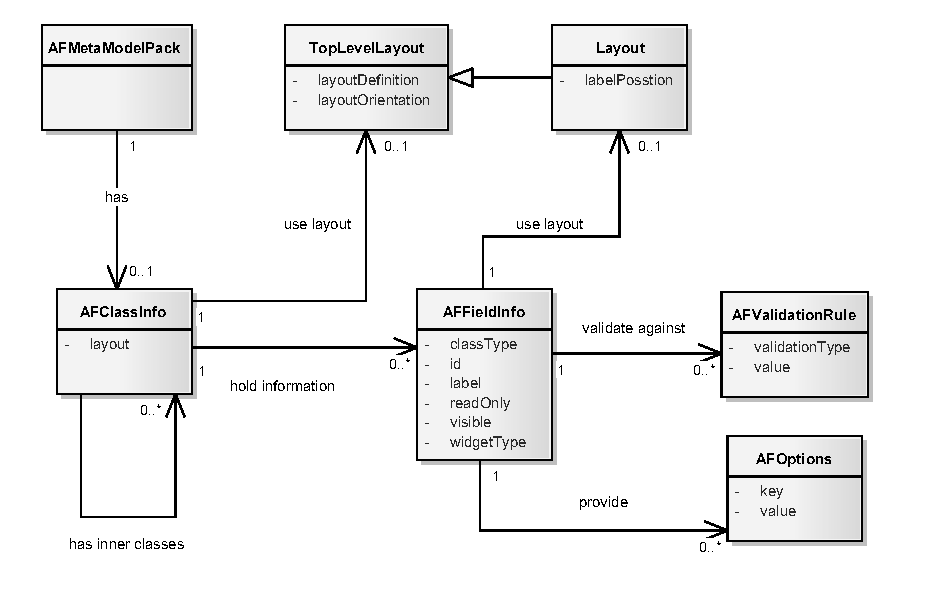
\includegraphics{images/domainModel}
\caption{Doménový model objektů obsahující metadata o objektu, nad kterým byla provedena inspekce}
\label{img:metadataModel}
\end{figure}

\subsubsection{AFMetaModelPack}
Tato třída zapouzdřuje informace, které popisují objekt, nad kterým byla prováděna inspekce. Třída rovněž slouží jako fasáda a nabízí programátorovi upravení metadat po generování. V případě serveru je toto návratový typ zdroje, na který klient přistoupí, chce-li znát metadata, která zdroj poskytuje.
\subsubsection{AFClassInfo}
Tato třída udržuje informace o hlavním objektu, z kterého je vytvářena definice. Třída má dále reference na své vnitřní proměnné a své potomky. Na základě generování dat je potřeba udržet pořadí, v kterém byla nad jednotlivými komponenty prováděna inspekce. V případě inspekce dat je i reference na neprimitivní datový typ jeho proměnná. Nicméně je potřeba, aby byl klient schopný určit, že se jedná o složitý datový typ a určit jeho pořadí v aktuálním objektu, aby mohl rozhodnout na jaké pozici objekt zobrazit. Z tohoto důvodu je ve třídě AFFieldInfo proměnná classType, která určuje, zdali se jedná o vnitřní třídu či primitivní datový typ.
\subsubsection{AFFieldInfo}
Tato třída je zodpovědná za poskytování detailních informací o proměnné objektu, nad kterým byla provedena inspekce. Třída udržuje název proměnné, widget, na který bude proměnná převedena, pravidla, která musí být splněna, název, pod kterým bude prezentována uživateli a zdali se jedná o složitý či jednoduchý objekt. Kromě těchto vlastností nese objekt také informace o tom, je-li komponenta viditelná a pouze pro čtení.
\subsubsection{AFRule}
Každá proměnná má souhrn vlastností, které musí být splněny. Typ widgetu ještě vždy nemusí určovat datový typ komponenty a neurčuje, je-li pole povinné či nikoliv. Tento soubor vlastností je popisován v této třídě. Třída využívá ENUM, který specifikuje podporované validace. Důvodem je to, že klient musí být schopný vytvořit tyto validační pravidla a interpretovat je na komponentě svým vlastním způsobem, který je specifický pro technologii, kterou používá. Jednou z dalších výhod je validace XML souboru, z kterého jsou pravidla vytvářena. Framework vytvoří pouze ty validační pravidla, která podporuje. Klient poté musí podporovaná pravidla interpretovat. 
\subsubsection{AFOptions}
Některé widgety umožňují, aby si uživatel vybral z několika předem připravených možností. Tyto možnosti musí být klientovi prezentovány. Tato třída udržuje informace o možnostech výběru v dané komponentě. Proměnná klíč je hodnota, která bude odeslána zpět na server a proměnná value je hodnota, která bude zobrazena klientovi. Tímto způsobem lze klientovi zobrazit jakýkoliv text, který bude zpětně mapován na jeho skutečnou hodnotu. Kromě textu lze samozřejmě zobrazit čísla či hodnoty výčtových typů.

\subsection{Server}
Server je zařízení či software, který umožňuje zpracovat požadavky od klientů a na jejich základě vytvořit odpověď. Server tedy poskytuje svým klientům určitý typ obsahu. Způsob a původ obsahu, který server poskytuje, je pro klienta povětšinou neznámý. V současné době je velmi populární přístup, při kterém server získá data z více zdrojů a poskytne je klientovi. Hovoříme o tzv. mashup \cite{Tuchinda2008}. Mashup nemusí být pouze z veřejných zdrojů, lze využít i privátní zdroje, či lze k sestavení odpovědi využít další služby. Klient napojený na server tohoto typu nemusí mít o těchto dalších zdrojích vůbec žádnou povědomost a dotazuje se pouze vůči tomuto serveru, který zpracovává jeho požadavky. 
Klientů, kteří získávají data z veřejných, či privátních zdrojů serveru může být celá řada. Mohou to být vlastní privátní aplikace, mobilní aplikace, Javascriptoví klienti či další server, který pouze využívá veřejné zdroje serveru k sestavení odpovědi svým vlastním klientům. V těchto případech je potřeba zvážit způsob generování definic dat, které by mohly způsobit stávajícím klientům problémy. V ideálním případě musí být framework integrován takovým způsobem, aby byla zachována stávající funkcionalita a framework ji pouze rozšířil. 
Ke generování definic objektů jsou potřeba následující věci:
\begin{enumerate}
\item Objekt, jehož definice budou generovány.
\item Mapování, na jehož základě bude rozhodnuto, o jaký typ komponenty půjde.
\item Definice komponenty včetně vlastností jako jsou validace, layout a popis chování komponenty.
\item Layout, ve kterém budou komponenty sestaveny.
\item Framework, který provede inspekci.
\item Framework, který bude inspekci řídit a bude interpretovat vygenerovaná data. Tento framework musí zároveň ověřit validitu jednotlivých komponent.
\end{enumerate}

Výše uvedené vlastnosti, nebudou mít vliv na změnu funkcionality. K inspekci a mapování bude využit framework AspectFaces \cite{aspectFaces}, který umožňuje na základě datových typů rozhodnout jakou komponentu využít. Definice komponent a jejich vlastností bude již v plné kompetenci vývojáře, nicméně základní komponenty a jejich chování bude předpřipraveno ve vzorovém projektu, aby se vývojář mohl inspirovat.

\subsection{Klient}
Klientská část frameworku bude vytvářet komponenty na základě metadat, která obdržela od serveru. Klient nebude mít žádnou znalost o objektech, které mu server poskytuje, předtím než obdrží jejich definice. Klient nicméně musí vědět, který zdroj mu poskytne relevantní definice a který ze zdrojů mu poskytne data odpovídající těmto definicím. Zároveň také musí vědět, na který zdroj data zpětně odeslat. Zdroj je obvykle specifikován následujícími parametry:
\begin{enumerate}
\item Adresa serveru
\item Port
\item Protokol
\item Metoda (get, post, put, delete)
\item Dodatečné hlavičkové parametry například content-type
\end{enumerate}
Klient tedy bude muset vždy specifikovat tyto parametry. Z hlediska použitelnosti je vhodné mít tyto specifikace v XML souboru, který bude umět klient jednoduše načíst. Pro usnadnění bude načítání provádět framework. Ukázka je na obrázku \ref{code:xmlSource}. V ukázkovém příkladu je specifikován zdroj s metadaty, který je vždy povinný. Zdroj se nachází na adrese\\ http://localhost:8080/AFServer/rest/users/loginForm. Zdroj s daty není specifikován, což způsobí, že ve formuláři nebudou žádná data. Formulář bude možné odeslat na adresu http://localhost:8080/AFServer/rest/users/login. Zdroj má identifikátor loginForm. V jednom XML dokumentu lze mít více zdrojů. K vložení dat do konkrétního zdroje lze využít EL. V hlavičce může být 0 až N parametrů, přičemž každý parametr musí být uveden ve stejném formátu, jako je znázorněno na obrázku \ref{code:xmlSource}. Obdobný způsob se využívá v JavaEE aplikací v deskriptoru web.xml. Klient umí sestavit požadavek na základě tohoto popisu a interpretovat odpověď od serveru. Není tedy nutné, aby uživatel implementoval třídy, které se umožní aplikaci připojení na server a získání dat.

\begin{lstlisting}[caption=Ukázka XML specifikace zdrojů,
label={code:xmlSource}, basicstyle=\footnotesize]
<?xml version="1.0" encoding="UTF-8"?>
<connectionRoot xmlns:xsi="http://www.w3.org/2001/XMLSchema-instance">
	<connection id="loginForm">
		<metaModel>
			<endPoint>localhost</endPoint>
			<endPointParameters>/AFServer/rest/users/loginForm</endPointParameters>
			<protocol>http</protocol>
			<port>8080</port>
			<header-param>
				<param>content-type</param>
				<value>Application/Json</value>
			</header-param>
		</metaModel>
		<send>
			<endPoint>localhost</endPoint>
			<endPointParameters>/AFServer/rest/users/login</endPointParameters>
			<protocol>http</protocol>
			<port>8080</port>
			<method>post</method>
			<header-param>
				<param>content-type</param>
				<value>Application/Json</value>
			</header-param>
		</send>
	</connection>
</connectionRoot>
\end{lstlisting}

Je patrné, že klient je schopný získat definice formulářů či tabulek, naplnit je daty a poté odeslat zpět na server. Důvodem, proč je klient schopný generovat formuláře na základě definice ze serveru je ten, že klient pracuje se stejnými objekty, které popisují metadata, jako server. Prozatím je k dispozici pouze strohý popis dat. Klientská část musí nyní rozhodnout jak data interpretovat, jak s nimi pracovat, jakým způsobem je validovat, jak je znovu sestavit a odeslat na server. Důležitým prvkem je i způsob uspořádání jednotlivých prvků, jejich velikosti, barvy a texty.

Využití frameworku by obdobně jako v případě serveru nemělo mít vliv na stávající použití aplikace. V případě referenčního řešení ve Swingu generuje klient JPanel, který lze vkládat do dalších panelů a vývojář tak není nikterak omezen, co se týče stávající aplikace. 

\begin{figure}[h!]
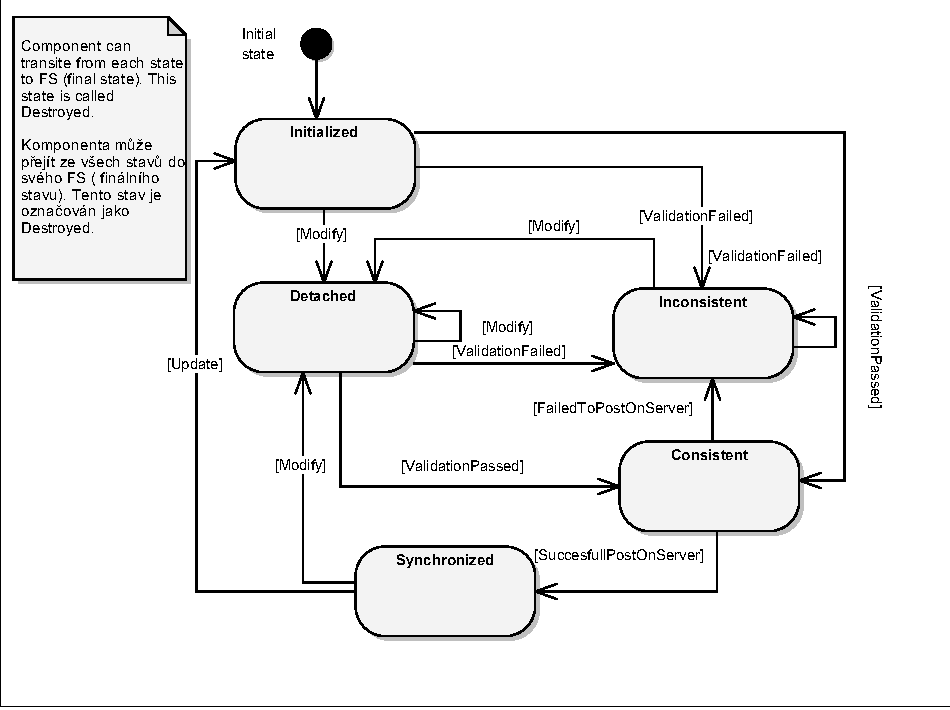
\includegraphics{images/formLifecCycle}
\caption{Životní cyklus formuláře}
\label{img:formLifeCycle}
\end{figure}

\subsection{Životní cyklus formuláře}
Formulář, jako každá komponenta, má svůj životní cyklus. Jeho stavy jsou znázorněny na obrázku \ref{img:formLifeCycle}. Formulář je po vygenerování a po naplnění daty v inicializačním stavu. V tomto stavu může být komponenta nevalidní, neboť data, která obdržela, nemusí splňovat požadované validace. K této situaci může dojít, je-li například přidána nová proměnná do datového modelu. Toto přidání obvykle probíhá tak, že se v koncové databázi, pokud jí software má, přidá políčko a nastaví se mu defaultní hodnota pro již existující data, která může být například null. V definici může být pole označeno jako povinné, avšak ve formuláři nemusí být vyplněno, což způsobí, že jsou data nevalidní, byť uživatel ve formuláři data nezměnil. Komponenta se pak přepne do stavu Inconsistent. V případě modifikace dat se komponenta dostává do stavu Detached. Tento stav značí, že byla data změněná. Pokud uživatel data stále mění, pak komponenta zůstává v tomto stavu. Ze stavu Detached přechází komponenta v případě úspěšné validace do stavu Consistent. V případě neúspěšné validace se komponenta dostane do stavu Inconsistent. Z tohoto stavu lze přejít pouze do dvou stavů jedním z nich je stav Detached. Do tohoto stavu lze přejít, pokud uživatel změní data ve formuláři. Komponenta může také zůstat ve stavu Inconsistent, pokud uživatel data nezmění a zkusí provést validaci znovu a tato validace opět selže. Konzistentní stav značí, že je komponenta připravená k odeslání dat na server. Pokud odeslání dat selže je komponenta přepnuta do stavu Inconsistent. V případě úspěšného odeslání dat, je komponenta přepnuta do stavu Synchronized. Ze stavu Synchronized lze přejít do stavu Initialized, pokud jsou data znovu načtena ze serveru a do stavu Detached, pokud jsou data upravena uživatelem.

\section{Případy užití}
Případy užití a jejich scénáře \cite{UmlArlow} specifikují chování systému. V této práci lze nahlížet na případy užití ze dvou stran. První z nich je koncový uživatel, neboli vývojář, který framework využívá. Druhým z nich je samotný framework, který provádí akce, aby splnil úkol, který mu uživatel uložil. V této sekci se zaměříme na případy užití koncového uživatele, které specifikují použití frameworku. Na obrázku \ref{img:useCase} jsou zachyceny všechny tyto případy užití. Pro ukázku detailně rozebereme případ užítí na obrázku \ref{img:useCaseSmall}. Na tomto případu je znázorněno odeslání dat z vygenerovaného formuláře zpět na server. Součástí je samozřejmě validace zadaných dat a jejich zpětné sestavení, neboť formulář byl vytvořen na základě metadat a klient tedy zná pouze strukturu objektu popsanou těmito metadaty. 
\begin{figure}[h!]
\begin{center}
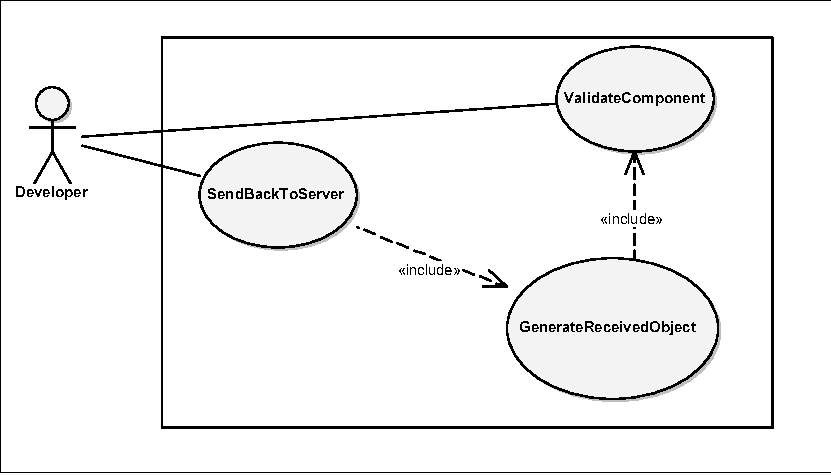
\includegraphics{images/useCaseSmall}
\caption{Část případů užití znázorňující odeslání dat na server z vygenerovaného formuláře}
\label{img:useCaseSmall}
\end{center}
\end{figure}
\subsubsection{Validace komponenty}
Tento případ užití je znázorněn na obrázku \ref{img:useCaseSmall} a jmenuje se ValidateComponent.

Případ užití: Validace komponenty\\
ID: 1\\
Popis: 
Uživatel využívá framework ke generování formulářů. Hlavním úkolem formuláře je možnost vkládat či upravovat data a odesílat je zpět na server. Před odesláním dat na server musí být provedena validace, aby se zajistilo, že bude formát dat serveru vyhovovat a bude umět s daty pracovat.
\\
Aktér: Uživatel\\
Vstupní podmínky:
\begin{enumerate}
\item Formulář musí být sestaven na základě metadat a framework musí znát formulář, s kterým chce pracovat.
\end{enumerate}
Scénář:
\begin{enumerate}
\item Případ užití začíná obdržením požadavku od uživatele žádající validaci dat.
\item Systém vyhledá pole k validaci.
\item Dokud existují pole k validaci pak:
\begin{enumerate}
\item Systém získá konkrétní pole k validaci.
\item Systém určí typ komponenty a požádá builder, který ji sestavil o data.
\item Dokud existuje validace, která zatím nebyla na poli vykonána pak:
\begin{enumerate}
\item Systém požádá validátor o validaci.
\item Pokud validace selže pak:
\begin{enumerate}
\item Systém ukončí validování tohoto pole a zobrazí u něj chybové validační hlášení.
\end{enumerate}
\end{enumerate}
\end{enumerate}
\end{enumerate}

Případ užití: Sestavení dat\\
ID: 2\\
Popis: 
Uživatel využívá framework ke generování formulářů. Hlavním úkolem formuláře je možnost vkládat či upravovat data a odesílat je zpět na server. Před odesláním dat na server musí být tyto data zpětně sestaveny, aby s nimi server dokázal pracovat.
\\
Aktér: Uživatel\\
Vstupní podmínky:
\begin{enumerate}
\item Formulář musí být sestaven na základě metadat a framework musí znát formulář, se kterým chce pracovat. Framework musí znát formát dat, která server očekává.
\end{enumerate}
Scénář:
\begin{enumerate}
\item Případ užití začíná obdržením požadavku od uživatele žádající sestavení dat z formuláře.
\item Zahrnout(Validace komponenty).
\item Pokud validace dopadla úspěšně pak:
\begin{enumerate}
\item Systém získá pole, která budou odeslána.
\item Pokud existuje pole, které ještě nebylo transformováno pak:
\begin{enumerate}
\item Systém určí typ komponenty a požádá builder, který ji sestavil, o data.
\item Systém určí název proměnné a třídu, do které patří, a nastaví jí data.
\end {enumerate}
\item Systém na základě formátu dat, které server očekává, rozhodne, v jakém formátu data zaslat a převede je na daný formát.
\end{enumerate}
\end{enumerate}

Výstupní podmínka:
\begin{enumerate}
\item Data ve formuláři byla převedena na objekt, s kterým umí server pracovat.
\end{enumerate}

Případ užití: Odeslání dat\\
ID: 3\\
Popis: 
Uživatel využívá framework ke generování formulářů. Hlavním úkolem formuláře je možnost vkládat či upravovat data a odesílat je zpět na server. Před odesláním dat na server musí být tato data zpětně sestavena, aby s nimi server dokázal pracovat, a musí splnit validační kritéria.
\\
Aktér: Uživatel\\
Vstupní podmínky:
\begin{enumerate}
\item Formulář musí být sestaven na základě metadat a framework musí znát formulář, se kterým chce pracovat. Framework musí znát zdroj, na který mají být data odeslána, a všechny potřebné informace, které zdroj vyžaduje.
\end{enumerate}
Scénář:
\begin{enumerate}
\item Případ užití začíná obdržením požadavku od uživatele žádající odeslání formuláře na server.
\item Zahrnout(Validace komponenty).
\item Zahrnout(Sestavení dat)
\item Dokud je validace či sestavení dat neúspěšné pak:
\begin{enumerate}
\item Systém zobrazí chybové hlášení a určí, u kterých polí nastala chyba.
\item Uživatel chybu opraví a požádá systém o opětovnou validaci a sestavení dat.
\end{enumerate}
\item Systém vytvoří připojení na specifikovaný zdroj a odešle data.
\item Pokud odeslání selhalo pak:
\begin{enumerate}
\item Systém zobrazí chybové hlášení, že nebylo možné data odeslat včetně odpovědi od serveru, je-li nějaká.
\end{enumerate}
\end{enumerate}

Výstupní podmínka:
\begin{enumerate}
\item Data byla odeslána.
\end{enumerate}


\section{Omezení frameworku}
Existují určité možnosti, které nebudou ve frameworku podporovány. V následujícím přehledu budou představeny nepodporované vlastnosti frameworku v aktuální verzi.
\begin{enumerate}
\item Inspekce datových proměnných typu List a Array
\item Získávání dat ve formátu XML. Framework plně podporuje JSON.
\item Customizace jednotlivých polí. Framework podporuje customizaci formuláře a všech jeho polí, nicméně nedisponuje možností přizpůsobovat jednotlivá pole.
\item Framework neumožňuje v jednom poli reprezentovat složený datový typ. Například třídu.
\item Odesílání dat a validace dat v tabulce. Tabulka je v této verzi pouze readonly.
\item Framework vyžaduje ke své funkčnosti jak serverovou tak klientskou stranu. V případě, že klientské straně chybí serverová strana, tak je framework nefunkční. V případě, že serverové straně chybí klientská strana, tak je serverová strana stále schopná vytvářet definice dat.
\item Klientská strana zobrazuje pouze ta data, která obdržela od serveru, nelze vytvářet automatický Mashup na klientovi. Nicméně klient může generovaný formulář umístit mezi jiné komponenty.
\item Klientská strana nedokáže sestavit objekt, který získala z metadat do takové míry aby z něj byla schopná vytvořit instanci. Neboli klientská strana si neudržuje konkrétní objekt, který obdržela, pouze jeho popis.
\item Serverová část využívá k automatické inspekci framework. Bez tohoto frameworku není možné inspekci provést, nicméně uživatel si může definovat svou vlastní definici bez nutnosti inspekce dat.
\end{enumerate}

\section{Uživatelé a zabezpečení}
Téměř každá aplikace využívá způsob, při kterém se uživatel autentizuje a aplikace mu na základě jeho rolí přidělí oprávnění. V případě využití bez stavového protokolu, jakým REST je lze posílat informace o uživateli v hlavičce požadavku. Tyto informace mohou být samozřejmě zašifrované. Framework podporuje vkládání libovolných informací do hlavičky requestu. Klient si také může zvolit, zdali bude využívat http či https protokol. Velmi rozšířenou možností je využitý Oauth. Jednou z možností, je vložení parametrů do hlavičky či do adresy. Vkládání dynamických adres či proměnných do hlavičky requestu framework podporuje. 

Druhou části jsou uživatelské role, na základě kterých se generuje uživatelské rozhraní. Serverová část využívá framework AspectFaces \cite{aspectFaces}, který podporuje uživatelské role v systému. Je jen na programátorovi, jaký framework na autentizaci a autorizaci na straně serveru použije. Jednou z možností je například napsat si vlastni interceptor, který určí, o jakého uživatele se jedná, přiřadí mu roli v systému, na základě které se mu zobrazí konkrétní obsah. Server při generování metadat může využít různé mapovací soubory na základě uživatelské role. Specifikace tohoto chování je opět v plné kompetenci uživatele.
\section{Použité technologie}
V následující sekci jsou rozebrány použité technologie. Kromě samotného frameworku je součástí práce i ukázkový projekt na platformě JavaEE a JavaSE.
\subsection{Java SE - Swing}
Klientská část frameworku je schopná vygenerovat formuláře či tabulky a naplnit je daty a data odeslat. Klientská část je přizpůsobena frameworku Swing. Důvodem je, že vývoj Swingové aplikace je rychlý a Swing zná velké množství vývojářů, kteří si framework mohou jednoduše otestovat. Nicméně metadata, která server generuje lze interpretovat v jakékoliv technologii. Swing je knihovna grafických a uživatelských prvků. Poskytuje komponenty, layouty, actionListenery, okna, dialogová okna a další prvky, pomocí kterých lze vytvářet interaktivní aplikace.
\subsection{Java EE}
Java EE je platforma sloužící k vývoji enterprise aplikací. V současné době je oblíbená jak u velkých tak u menších korporací. Java EE přináší podporu pro Restové služby, JFS, JSP, EJB, databázové frameworky, anotace a další komponenty. Aplikace v JavaEE se obvykle nasazuje na aplikační server. Aplikační servery mohou být v cloudu a podílet se společně na zpracování requestů. Důvodem využití této platformy je fakt, že klient vytváří requesty vůči serveru a server tato data zpracovává. Je vhodné mít na serveru platformu, která je ověřená a má potenciál ke zpracování těchto requestů. V této práci generujeme data pomocí restového rozhraní a Java EE splňuje specifikaci, které se tohoto rozhraní týká. 
\subsection{AspectFaces}
AspectFaces je framework, který umí provádět inspekci nad zadanými objekty a na základě datových typů a dalších parametrů rozhodovat o to, jaká komponenta se použije pro konkrétní datový typ. Framework využívá AspectFaces k tomu, aby provedl toto mapování a sestavil popis uživatelského rozhraní. Hlavním důvodem využití tohoto frameworku je fakt, že je distribuován jako open source pod licencí LGPL v3 a že lze využít jeho funkcionalitu ke statické inspekci dat. Tato inspekce je již odladěna a není tedy důvod psát znovu již vynalezenou věc. 
\subsection{Ukázkový projekt}
Ukázkový projekt demonstruje použití frameworku. Skládá se ze dvou částí. Klientské a serverové. Klientská část využívá pouze Swing. Serverová část je mnohem sofistikovanější a využívá aktuální technologie. Ukázkový projekt zde znázorňuje použítí frameworku a jeho omezení. Ukázkový projekt je koncipován, tak aby ho bylo možné nasadit bez nutnosti dodatečného nastavení.
\subsubsection{GlassFish}
GlassFish \cite{glassfish} je open source aplikační server, jedná se o certifikovaný server JavaEE. Umožňuje clustering, monitoring, podporu EJB, REST a JDBC. Architektura jádra je založena na frameworku OSGI, který umožňuje vzdáleně přidávat, startovat či ukončovat komponenty bez nutnosti restartování celého serveru. Důvodem proč je Glassfish využit na tomto projektu je čistě demonstrativní. Nicméně, každý aplikační server má svá specifika, a proto je ukázková aplikace odladěna právě pro GlassFish. Jak již bylo zmíněno Glassfish distribuje vestavěnou podporou pro Rest a umožňuje použití Derby DB v režimu in-memory bez nutnosti speciálního nastavení.
\subsubsection{RestEasy}
Jedná se o framework, pomocí kterého lze vytvářet RESTful aplikace. Tento framework může běžet v libovolném servletovém kontajneru. Framework podporuje například JSON, XML serializace objektů, EJB a je splňuje JAX-RS implementaci. Tvorba aplikací s restovým rozhranním je tak díky tomuto frameworku mnohem jednodušší a vývoj je rychlejší. 
\subsubsection{EJB}
Enterprise JavaBeans \cite{javaEETutorial} jsou serverově orientované komponenty, které zapouzdřují business logiku a přístup do databáze. Jsou spravovány v rámci serverového kontejneru, který zajišťuje jejich vytvoření i odstranění z paměti. EJB mohou být různých typů.
\begin{itemize}
\item Stateless
\item Statefull
\item Singleton
\end{itemize}
Jak již bylo zmíněno, o jejich správu se stará serverový kontejner, nemusíme tedy řešit problémy spojené s vytvořením a destrukcí singletonu \cite{gamma}. Mezi hlavní výhody EJB patří transakční zpracování, zajištění systémových služeb a bezpečnostní autorizace. Abychom definovali či~získali přístup k těmto třídám, používáme anotace, které jsou velmi dobře čitelné a~srozumitelné.
\subsection{Derby DB}
V ukázkovém projektu je potřeba data ukládat do databáze. Při vytváření byl kladen důraz na to, aby noví uživatelé nemuseli v konfiguračních souborech specifikovat nastavení a mohli ukázkový projekt ihned nasadit a vyzkoušet. Z tohoto důvodu je využita light databáze Derby. Ukázkový projekt ji využívá v in-memory módu, což znamená, že budou data po zastavení serveru ztracena. Spolu s Derby DB využívá ukázkový projekt ORM s defaultním nastavením na create. Po startu aplikace jsou v čisté databázi vytvořeny požadované tabulky, které odráží definice objektů, jenž jsou anotované jako entity. Další výhodou je možnost využít anotací k nastavení validací přímo na databázi. Tyto validace pak mohou být využity při inspekci dat a na jejich základě mohou být vytvořeny validace, či konkrétní komponenty.
\chapter{Implementace}
\section{Architektura}
Jak už bylo popsáno, tato práce se zabývá tvorbou dvou klienstkých frameworků pro dvě různé mobilní platformy. Ke správnému fungování frameworků je předpokládána serverova část, která generuje data v určité struktuře a formátu, z nichž oba frameworky umí vytvořit a zobrazit koncovému uživateli prvky grafického uživatelského rozhraní. Použití frameworku na jednotlivých zařízeních zachycuje diagram nasazení na obrázku \ref{img:deploymentDiagram}. Diagram nasazení je určen k tomu, aby zobrazil jak je architektura softwaru namapovaná na architekturu hardwaru. Jedná se o diagram, který patří do implementační fáze, avšak často již vzniká určitá první verze ve fázi návrhové a poté se doplňuje \cite{UmlArlow}.

Obrázek \ref{img:deploymentDiagram} zobrazuje tři zařízení - server, Android klienta a Windows Phone klienta. Pro účely vývoje těchto frameworků byla na serveru nasazena Java EE aplikace AFServer, která za pomocí AFRest \cite{tomasek-thesis} využívající AspectFaces \cite{aspect-faces} generuje definice komponent z modelu, které pak upraví a poskytuje klientovi v požadovaném tvaru, který ji může získat pomocí http dotazu. Android klient interpretuje tuto specifikaci komponenty za pomocí frameworku AFAndroid, který využívá stejných částí jako serverová strana, což zajišťuje kompatibilitu objektů na serverové a klienstké straně. Windows Phone klient interpretuje definici za pomocí AFWinPhone, který bohužel neumožňuje využívat stejných částí se serverem neboť běží na rozdílných platformách. Aby bylo zachováno stejné chování jako u Android klienta, byly tyto části znovu vytvořeny.

Aby klienti mohli framework využívat, musí ho nejdříve vložit. V případě Androidu se framework kompiluje do AAR souboru, který lze do projektů přidat jako Gradle závislost. Gradle je systém pro build projektů a správu závislostí nejen v Androidu. V současné době ho lze využít i v C, C++, Java aplikacích \cite{gradle}. Závislost může být lokální nebo se stahovat z online repozitáře. Jelikož není AFAndroid ještě k dispozici v žádném z online repozitářů, je nutné ho přidat lokálně. To lze udělat přidáním AAR souboru do složky lib nebo vytvořit z knihovny nový modul. Windows Phone framework je zase zkompilován do DLL souboru, který je v současné chvíli nutné také přidat lokálně jako knihovnu mezi reference.

\subsection{Komponenty}
Oba frameworky jsou schopny generovat dva typy komponent - formulář a list. Obě tyto komponenty dědí od třídy AFComponent, která představuje společnou část obou komponent. AFComponent implementuje rozhraní třídy AbstractComponent, která definuje metody pro získání definice komponenty, naplnění daty, generování dat pro odeslání a jejich odeslání na server včetně validace. Tyto metody musí AFComponent nebo některá třída, která od něj dědí, nuceně implementovat. Společná část komponent konkrétně implementuje metody pro získání definice ze serveru a získání dat, kterými se má komponenta naplnit, protože tyto části jsou jak pro formulář, tak pro list identické. Způsob reprezentace komponenty a vložení získaných dat, pak řeší jednotlivé komponenty každá jiným způsobem. Stejně tak list nedisponuje stejnou funkcionalitou jako formulář, je jen pro čtení a proto nepodporuje metody pro generování a následné odesílání dat či jejich validaci. Struktura části Android frameworku zachycující komponenty je na obrázku \ref{img:classDiagramComponents} popsána diagramem tříd. Diagram pro tuto část ve Windows Phone frameworku je až na syntaktické odlišnosti shodný.  

Obě komponenty obsahují metodu, která získá jejich grafickou reprezentaci, kterou pak může vývojář vložit do libovolné části uživatelského rozhraní, neboť tato metoda má návratový typ u Android verze View a u WP verze FrameworkElement, což jsou jedny ze základních prvků GUI na těchto platformách a lze je vložit do jakéhokoliv jiného elementu. V AFSwinx \cite{tomasek-thesis} komponenty rovnou dědily od třídy JPanel a tudíž metodu pro zisk grafické reprezentace nepotřebovaly. Tento přístup však vyústil v to, že se metody poskytované komponentou mísily s nepřeberným množstvím metod příslušících třídě JPanel, což způsobovalo dle uživatelského testu nepřehlednost a zhoršenou orientaci v poskytovaných metodách, proto byl zvolen výše zmíněný přístup. 

Vytvářené komponenty se ve frameworku určitým způsobem ukládají, aby bylo možné je získat a pracovat s nimi v celém programu, ne jen v místě, kde byly vytvořeny. Konkrétně se komponenty skladují ve třídách AFAndroid pro Android a AfWindowsPhone pro WP, zobrazené na obrázku \ref{img:facades}. Tyto třídy jsou implementovány jako singleton, což je návrhový vzor, který se využívá, když je potřeba mít pouze jednu instanci této třídy, ke které lze přistupovat z více míst \cite{gamma}. Singleton často bývá součástí jiných návrhových vzorů jako je napříkald Facade neboli fasáda. Fasáda se používá v případě, že programátor chce poskytnout jednoduché rozhraní pro ovládání složitějšího systému a tím klienty odstínit od vnitřní implementace systém schovaného pod fasádou \cite{gamma}. AFAndroid a AFWinPhone tedy neslouží pouze jako sklad vytvořených komponent ale také jako fasády pro ovládání frameworků. Nabízí získání vytvořené komponenty, jejich smazání, zisk builderů pro tvorbu komponent a nastavení základního skinu, který se použije při sestavování komponent, není-li v při inicializaci builderu specifikováno jinak. Proces sestavení komponenty je složitější proces několika funkcí, které na sebe musí navazovat ve správném pořadí, proto kdyby tyto třídy neexistovaly, nebylo by použití frameworků vůbec snadné.

\begin{figure}[h!]
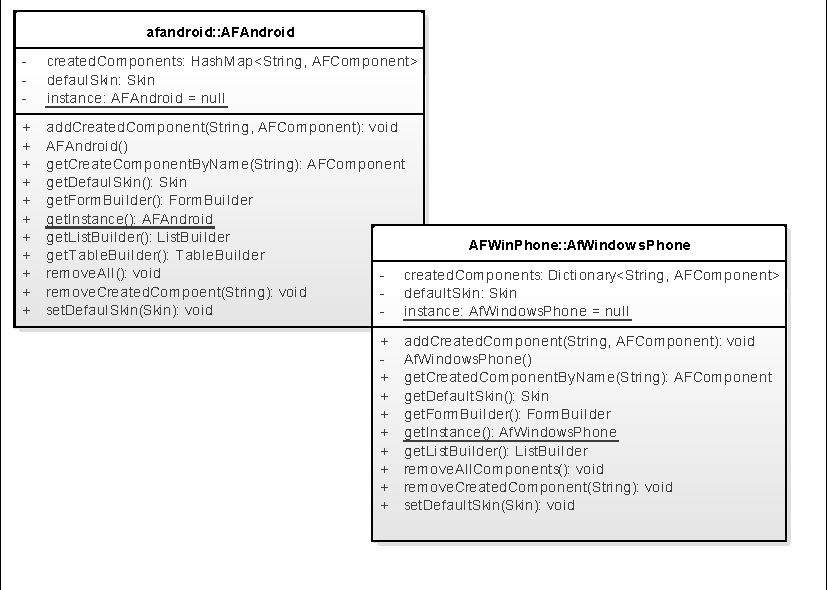
\includegraphics[width=\textwidth]{figures/facades}
\caption{Třídy AFAndroid a AfWindowsPhone sloužící jako fasády pro ovládání frameworků}
\label{img:facades}
\end{figure}

Přiklad vytvoření komponenty v Android frameworku, konkrétně formuláře, za použití fasády AFAndroid je v ukázce kódu \ref{code:createForm}. Kód ukazuje, že je třeba za použití fasády získat builder, který je pak nutné nainicializovat. Inicializace zahrnuje určení zdroje, ze kterého se má definice komponenty získat, definuje InputStream s načteným souborem s definicemi zdrojů a klíč, pod kterým se získá konkrétní připojení. Soubor byl popsán v rámci analýzy a jeho struktura je ukázána v části kódu \ref{code:xmlSource}. Vývojář si komponentu také při inicializaci builderu pojmenuje, tedy přiřadí ji jednoznačný textový řetězec, pod kterým se komponenta uloží do vytvořených komponent a na základě tohoto řetězce ji lze odtud skrz fasádu opět získat. Existuje ještě přetížená metoda pro inicializaci builderu, která je umožnuje přidat dodatečná nastavení pro připojení. Po inicializaci builderu lze nadefinovat ještě skin, který se při vytváření komponenty použije. Jelikož je komponeta vytvářena dynamicky všetně jejích vlastností a vzhledu v rámci metody, která je pro vývojáře zapouzdřená, jediným způsobem jak pohodlně upravit její vzhled je nastavit skin před zahájením její tvorby. Jelikož má vývojář k některým částem komponenty přístup i po jejím vytvoření, lze vzhled komponenty upravit i později, vyžaduje to však znalosti tvorby GUI pro danou platformu, což už je složitější záležitost. Po nastavení skinu lze komponentu vytvořit a dále pak nad ní provádět akce, které poskytuje.  Pro Windows Phone je kód identický, pouze se používá WP fasáda AfWindowsPhone a místo InputStreamu stačí nadefinovat jméno souboru se zdroji, respektive cesta k němu.

Pokud se něco při vytváření nepovede,  například se nelze připojit ke zdroji na serveru, je vyhazována výjimka. Vývojář může výjimku libovolně zpracovat, například zobrazit dialog s chybou.

\begin{lstlisting}[caption=Ukázka tvorby formuláře,
label={code:createForm}, basicstyle=\footnotesize]
InputStream connectionResource = getResources().openRawResource(R.raw.connection);
 try {
	AFForm form = 
		AFAndroid.getInstance().getFormBuilder()
		.initBuilder(getActivity(), LOGIN_FORM_NAME, connectionResource, 
		LOGIN_FORM_CONNECTION_KEY)
		.setSkin(new LoginSkin(getContext()))
		.createComponent();
} catch (Exception e) {
	zpracovani vyjimky, ktera mohla nastat pri vytvareni komponenty
}
\end{lstlisting} 

\section{Komunikace serveru a klienta}
Jak už bylo zmíněno v analýze, server poskytuje zdroje, ze kterých lze získat definice komponent, data nebo na ně lze odeslat uživatelský vstup. K nadefinování těchto zdrojů je potřeba vytvořit XML soubor, který je popsán v ukázce kódu \ref{code:xmlSource}. Tento soubor se zpracuje pomocí příslušného XML parseru a výsledkem je třída AFSwinxConnectionPack, která má v sobě uloženy jednotlivé části daného připojení, kokrétně, kde je uložena definice komponenty, data a kam lze odeslat uživatelský vstup \cite{tomasek-thesis}. V průběhu tvorby komponenty se tyto části připojení využijí k zisku informací, které jsou na definovaných zdrojích, na něž připojení odkazuje, uloženy. Zisk informací je proveden pomocí HTTP požadavku, který vytváří a odesílá třída RequestMaker. Způsob provedení tohoto požadavku je na obou platformách dosti rozdílný, avšak něco mají společného a to, že musí být asynchronní. V mobilních aplikacích se requesty musí provádět asynchroně na jiném vlákně než na hlavním, neboť hlavní vlákno spravuje celé UI aplikace a to by v momentě, kdy se požadavek provádí, zamrzlo, což je nežádoucí. HTTP požadavek v případě, že se získává definice komponenty nebo data, vrací textový řetězec, který obsahuje JSON objekt převedení na textovou reprezentaci, v případě odesílání na server se akce pouze provede.

V Androidu se standartně HTTP requesty řeší v rámci objektu typu AsyncTask \cite{asynctask}, který umožňuje provést akci v pozadí a výsledky akce předat hlavnímu UI vláknu. Tím se vývojáři Android aplikací vyhnou přímé práci s vlákny. Třída RequestMaker od AsyncTask dědí a přetěžuje metodu pro práci v pozadí, kde se celý požadavek vytvoří, odešle a získá se odpověď. Tvorbu a práci s požadavkem má na starosti třída HttpURLConnection, před Android 6.0 by bylo možné ještě použít Apache HttpClient, který byl s příchodem nové verze Androidu smazán. Lze ho po určitém nastavení nadále používat ale ukazuje se, že HttpURLConnection je efektivnější z hlediska využití sítě a spotřeby energie \cite{httpclientremoval}. 

Specifikace požadavku, tj. http metoda, url adresa, data, content-type a případně bezpečnostní omezení, se předávají třídě v konstruktoru. Během procesu se může stát výjimka a jelikož metoda, která pracuje na pozadí nemůže zpropagovat výjimku o úroveň výš, je nutné výjimky řešit v rámci zmíněné metody. Je ale žádoucí ponechat řešení těchto výjimek na vývojáři, proto byla zavedena alternativa, ve které metoda běžící na pozadí vrací Object, který buď může být textový řetězec s daty ze serveru nebo vzniklá výjimka. O úroveň výše tento fakt kontroluje a v případě, že se jedná o výjimku, je vyhozena a zpropagována až k vývojáři. 
Po vytvoření objektu RequestMaker je třeba ho spustit. K tomu slouží metoda executeOnExecutor, která umožňuje spustit v jednu dobu více objektů typy AsyncTask.

WindowPhone verze používá k tvorbě a manipulaci s požadavkem třídu HttpClient \cite{wp-httpclient} v rámci asynchronní metody, která request provádí. V tomto případě problém s propagací případné výjimky až k vývojáři. Nastavení požadavku se provádí přes konstruktor obdobně jako v Android verzi. 

\subsection{Generování komponent}
Na základě definice komponenty, která se ze serveru získá výše uvedeným způsobem, lze generovat komponenty. Typ komponenty, která se vygeneruje závisí na zvoleném builderu. Každý builder je reprezentován třídou, která dědí od abstraktní třídy AFComponentBuilder. Tato třída definuje společné vlastnosti všech builderů a  vynucuje implementaci metody pro vytvoření komponenty jako takové a vytvoření její grafické reprezentace. Proces vytvoření komponenty v Android frameworku je popsán na sekvenčním diagramu v příloze \ref{img:sdFormBuilding}. Proces tvorby ve WP verzi je obdobný s tím rozdílem, že není potřeba znát k vytváření GUI prvků kontext, proto nemusí být do argumetů funkcí předávána aktivita, ve které chceme komponentu vytvořit. Z obrázku je patrné, že po inicializaci builderu a případném nastavení skinu začíná proces tvorby formuláře na jehož konci uživatel získá již hotový formulář. Nejprve dojde k získání metamodelu komponenty ze serveru. Poté začne tvorba jednotlivých polí formuláře, k tomu je zapotřebí odpověď s metamodelem rozparsovat, výsledkem čehož bude třída AFClassInfo obsahující informace o celé komponentě. Tato struktura byla v analytické části popsána na obrázku \ref{img:metadataModel}, skutečná struktura v tomto případě pro Windows Phone framework je na obrázku \ref{img:metadataClass}. AFClassInfo obsahuje 0 až N objektů třídy FieldInfo, tedy objektu držící informace o tvořeném poli. Přes tyto objekty framework iteruje a postupně z nich vytváří objekty třídy AFField, které už obsahují i grafickou reprezentaci pole. 

Při iterování skrze popisy polí je důležité kontrolovat atribut, který určuje zda pole zastupuje v modelu na serveru primitivní nebo složený datový typ. V případě, že se jedná o složený datový typ, vyhledá se k němu v AFClassInfo příslušná definice vnitřní třídy, na kterou se pak funkce, která tvoří jednotlivá pole, rekurzivně zavolá a na místo pole označeného jako vnitřní třída budou vytvořena pole, která jsou nadefinovaná v příslušné vnitřní třídě. 

Součástí tvorby pole není jen nadefinování vlastností a tvorba samotné grafické reprezentace. Při tvorbě formulářových polí je potřeba vytvořit tři elementy, ze kterých se pole skládá - label, místo pro zobrazení validačních chyb a aktivní prvek. To zajišťuje třída FieldBuilder. Vytvořit label a místo pro validační chyby je jednoduché, aktivní prvek je mírně komplikovanější. Součástí třídy FieldInfo je i atribut widgetType, který určuje, jakým typem aktivního prvku má být pole reprezentováno. Na základě tohoto atributu se získává pomocí třídy WidgetBuilderFactory příslušný builder, který umí přímo příslušný aktivní prvek vytvořit. Tento builder poskytuje také funkcionalitu pro získání a nastavení dat vytvořenému aktivnímu prvku. Pro jednoduší přístup k této funkcionalitě, má pole formuláře na builder, který mu vytvořil část s aktivním prvkem, referenci. Po vytvoření všech tří částí se zkompletují do celkové grafické reprezentace, která se poli taktéž nastaví. Takovéto pole se vrátí builderu komponenty, který si jeho existenci zaznamená. Po zaznamenání všech polí, které mají ve formuláři být, se jednotlivé grafické reprezentace polí seskupují do celkového vzhledu komponenty, který se pak komponentě nastaví a vývojář ho potom může z komponenty získat.

\subsubsection{Naplnění komponety daty}
Pokud má být komponenta naplněna daty, je nutné získat jednotlivé buildery, které vytvořily jenotlivá pole. Data se vkládají přímo z odpovědi serveru, která je obsahuje. V datech se objevuje vždy identifikátor daného pole a hodnota, která má být vložena. Dle tohoto identifikátoru je framework shopen vyhledat příslušné pole a z něj získat builder, který postavil jeho aktivní část. Jak už bylo řečeno, builder disponuje funkcí schopnou do pole, které vytvořil, vložit data, což také provede. Takto se to provede u všech polí, která se v přijatých datech vyskytují. Tím je proces tvorby formuláře popsaného na obrázku \ref{img:sdFormBuilding} ukončen a vývojáři je předána vytvořená komponenta. 

\subsubsection{Widget buildery}
Bylo zmíněno, že části formulářových polí, do kterých lze zadat uživatelský vstup, se vytváří pomocí příslušných builderů, jež lze získat pomocí třídy WidgetBuilderFactory. Tato třída využívá návrhový vzor Factory. Ten se využívá, když je potřeba vytvořit objekt a zároveň zastínit logiku vytváření objektu klientovi \cite{factorypattern}. Tento návrhový vzor byl ve frameworku použitý proto, aby se v případě, že by bylo potřeba přidat nový builder, nezasahovalo do logiky vytváření polí, ale pouze do třídy WidgetBuilderFactory. Jednotlivé widget buildery lze vidět na obrázku \ref{img:factoryWidgetBuilders} a jejich seznam je v tabulce \ref{table:widgetBuilders}. Každý builder dědí od základního builderu definovaného abstraktní třídou BasicBuilder implementující rozhraní AbstractWidgetBuilder. AbstractWidgetBuilder definuje metody pro vytvoření grafické reprezentace widgetu, nastavení dat do widgetu a zisk dat z widgetu. Tyto metody musí být pak každým novým builderem implementovány. Ukázka kódu \ref{code:createTextField} zobrazuje tvorbu grafické reprezentace textového pole v Android frameworku.

\begin{lstlisting}[caption=Ukázka tvorby grafické reprezentace textového pole,
label={code:createTextField}, basicstyle=\footnotesize]
@Override
public View buildFieldView(Activity activity) {
    EditText text = new EditText(activity);
    text.setTextColor(getSkin().getFieldColor());
    text.setTypeface(getSkin().getFieldFont());
    addInputType(text, getField().getFieldInfo().getWidgetType());
    if(getField().getFieldInfo().getReadOnly()){
	text.setInputType(InputType.TYPE_NULL);
        text.setTextColor(Color.LTGRAY);
    }
    return text;
}
\end{lstlisting} 

V ukázce \ref{code:createTextField} lze vidět, že na vstupní pole je aplikován skin, který upravuje jeho vzhled. Konkrétně v případě textového pole se nastavuje barva jeho textu a typ písma.

\begin{table}[h!]
\begin{center}
\caption{Podporované widget buildery}
\label{table:widgetBuilders}
\begin{tabular}{|p{4cm}|p{3cm}|p{7cm}|}
\hline
\textbf{Builder} & \textbf{Typ widgetu} & \textbf{Popis} \\
\hline
DateWidgetBuilder & 
Calendar & Používá se při reprezentaci atributů typu datum. Umožní uživateli zobrazit date picker, pomocí kterého lze vybrat datum. \\
\hline
DropDownWidgetBuilder &
dropDownMenu & Menu, ze kterého lze vybrat jednu z několika voleb. \\
\hline
CheckBoxWidgetBuilder & checkBox &
Zaškrtávací políčko reprezentující hodnotu true nebo false podle toho, zda je nebo není zaškrtnuto. \\
\hline
TextWidgetBuilder & textField &
Builder pro textové pole. Lze mu nastavit typ vstupu, podle kterého se změní klávesnice pro zadávání znaků například na číselnou. V Android frameworku lze použít i pro pole s heslem. \\
\hline
PasswordWidgetBuilder & password &
Pole pro hesla. Text, který uživatel dovnitř napíše je převeden na zástupné znaky. Tento builder se vyskytuje pouze ve WP verzi frameworku, Android verze k tomuto účelu používá TextWidgetBuilder \\
\hline
OptionBuilder & option &
Vytvoří skupinu radiobuttonů, z které lze vybrat jednu hodnotu. Pokud nejsou definovány možnosti vytvoří se 2 radiobuttony s hodnotami ano a ne \\
\hline
\end{tabular}
\end{center}
\end{table}

\subsubsection{Skiny}
Skiny neupravují pouze vzhled aktivního prvku, ale také vzhled labelu, validačních chyb nebo i celé komponenty. Lze nastavit grafické vlastností jako je barva textu, pozadí, velikost textu a jeho font, ale také rozměry celé komponenty. Ve frameworcích existuje rozhraní Skin, které deifnuje všechny nastavitelné vlastnosti. Už bylo zmíněno, že skiny se musí nastavit před tvořením komponenty jejímu builderu. Toto nastavení je ale volitelné a tak existuje třída DefaultSkin, která toto rozhraní implementuje a definuje základní vzhled, který se použije nespecifikuje-li vývojář jinak. Vývojář pravděpodobně nebude chtít předělat úplně celý vzhled, ale ppuze některé části skinu. K tomuto mu stačí dědit od třídy DefaultSkin a pouze přetížit metody udávající vlastnosti, které chce změnit.

\subsubsection{Layouty}
Při vytváření grafické reprezentace komponenty, server definuje, jak se její jednotlivé části v rámci komponenty uspořádají. V případě formuláře je nutné uspořádat pole tak, aby byl formulář přehledný a dobře použitelný. V případě listu jde hlavně o přehlednost, neboť jednotlivé položky listu by byly při větším obsahu moc vysoké a nevzhledné. Server definuje osu, podle které jsou komponenty vykreslovány, počet sloupců a pozici labelu \cite{tomasek-thesis}. Layout lze určit buď celé komponentě, ten na obrázku \ref{img:metadataClass} reprezentován třídou TopLevelLayout nebo pouze části komponenty tj. poli, který je na obrázku reprezentován třídou Layout. V případě layoutu komponenty je pouze definována osa a počet sloupců, layout jednotlivých polí přidává pozici labelu. Hodnoty, kterých jednotlivé vlastnosti nabývají jsou popsány pomocí následujících výčtových typů, které lze vidět i na obrázku \ref{img:metadataClass}.
\begin{itemize}
\item LayoutDefinitions, který určuje počet sloupců a nabývá hodnot ONECOLUMNLAYOUT a TWOCOLUMNSLAYOUT, tedy jednosloupcové a dvousloupcové rozložení.
\item LayoutOrientation, který určuje osu, ve směru které se části komponenty vykreslují. Nabývá hodnot AXISX a AXISY, první určuje směr vykreslování podle osy X, druhá podle osy Y.
\item LabelPosition, který určuje pozici labelu vzhledem k aktivnímu prvku. Nabývá hodnot BEFORE, AFTER a NONE. První znamená, že bude label před aktivním prvkem, druhá za aktivním prvkem a třetí znamená, že label nebude vůbec zobrazen.
\end{itemize}

Layouty jsou v jednotlivých klientských frameworcích interpretovány různě. Zatímco v případě Android frameworku je layout realizován pomocí seskupení LinearLayoutů \cite{android-lin-layout}, WP verze používá k tvorbě layoutu Grid \cite{wp-grid}. Důvodem není nic zvláštního, k oběma třídám existují na druhé platformě ekvivalenty, pomocí kterých lze dosáhnout stejných výsledků, jde spíše o to, ukázat více možných způsobů implementace. 

Důležitým aspektem je také pořadí jednotlivých částí komponenty. To definuje server a v metadatech se informace o polích objeví už v daném pořadí, které je třeba zachovat. Proto bylo nutné použít k uskladnění kolekci, která zachovává pořadí svých prvků, takovou je například List \cite{tomasek-thesis}.

\subsubsection{Lokalizace}
Jelikož se mohou v metadatech objevit i texty pro překlad, bylo třeba naimplementovat třídu Localization, která se stará o překlady těchto textů. Třída disponuje samoutnou funkcí pro překlad a funkcí pro změnu jazyku. V Androidu se typicky lokalizační texty umisťují do souboru strings.xml ve složce values. Pro Windows Phone je to obdobné. Zde se texty vkládají do souborů Resources.resw, které jsou umístěny ve složce s názvem jazyku ve složce Strings. S tímto umístěním textů oba frameworky počítají, u Android verze je sice možnost nadefinovat jiný balíček, ve kterém by se texty měly hledat, ale stále se předpokládá umístění ve values/strings.xml. Třída Localization se dá využít i pro překlad jiných textů i mimo framework a to i v rámci XML šablon, ve kterých je vytvořeno statické UI. Při startu aplikace se použije jazyk zařízení. Pokud by pro daný jazyk neexistovaly předklady, je vhodné mít defaultní soubory s texty, které se v tomto případě použijí.

\subsection{Práce s komponentami}
Vytvořená komponenta disponuje různými funkcemi, které umožňují s ní dále pracovat. Pro formulář jsou to metody pro odeslání, validaci, resetování nebo vyčištění formuláře. List je komponenta, která by měla pouze zobrazovat data, proto s ní nejde provést ani moc akcí. Obsahuje však důležitou funkci, pomocí které lze získat obsah jedné položky listu, který lze pak využít například pro naplnění formuláře. 

Nejdůležitější funkcí je však odeslání formuláře, který je zobrazen na sekvenčním diagramu \ref{img:sdFormSend}. K tomuto účelu má formulář metodu sendData. V rámci této metody se nejdříve zjistí, zda vývojář pro komponentu nadefinoval v XML souboru s připojeními část označenou uzlem <send>, který definuje, kam se budou data odesílat a jehož struktura lze vidět v ukázce kódu \ref{code:xmlSource}. Komponenty mají atribut connectionPack typu AFSwinxConnectionPack, který obsahuje všechna definována připojení. V případě, že vývojář specifikoval uzel <send> se v tomto atributu formuláře objeví i připojení na zdroj, který přijímá uživatelský vstup. Pokud připojení nadefinované není vyhodí se výjimka, která je propagována k vývojáři, který s ní dle svého uvážení naloži. Pokud připojení existuje, vygenerují se z formuláře data ve formátu, které server dokáže zpracovat. Klient nezná přesně objekty, které se odeslání na serveru vytvoří či upraví, zná ale jejich strukturu, která stačí k tomu, aby byla vytvořena data, která server dokáže přijmout. V rámci generování dat proběhne nejdříve jejich validace, která je blíže popsána v sekci níže. Pokud data nejsou validní vrací metoda sendData hodnotu false, která určuje, že se odesílání nezdařilo. Samotný proces generování dat byl převzat z frameworku AFSwinx. Ten využívá pro znovupostavení dat object typu BaseRestBuilder disponující metodou reserialize. \cite{tomasek-thesis}. BaseRestBuilder je implementován prozatím jen třídou JSONBuilder, která dokáže z formuláře vytvořit JSON soubor a použije se v případě, že server požaduje JSON formát. Další formáty nejsou prozatím podporovány. Metoda reserialize, kterou builder dat používá, již očekává vyparsovaná data z komponenty uložená v objektu typu AFDataHolder. Vytvoření těchto dat provádí komponenta sama. Uživatelský vstup získává z aktivní prvků, ke kterým má skrz kolekci polí typu AFField přístup. Data se získávají z aktivního prvku pomocí widget builderu, který aktivní prvek vytvořil a na který má AFField referenci.  Každý AFField má svůj unikátní identifikátor, který lze využít pro zjištění pozice proměnné v objektu na serveru, který má odeslání formuláře ovlivnit. Pokud indentifikátor obsahuje tečku, znamená to, že dané pole je částí reprezentace neprimitivního datového typu, tedy vnitřní třídy a k té je třeba hodnotu promenné přidat. Pokud v identifikátoru tečka není, znamená to, že jsme na správném místě a do mapy AFDataHolder se přidá nová proměná s hodnotou \cite{tomasek-thesis}. Android verze využívá již naimplementovaný JSON Builder, který využívá k sestavení dat framework GSON \cite{gson}.Ve Windows Phone verzi musel být builder dat přepsán a využívá Windows knihovnu pro práci s JSON soubory. Po vytvoření dat stačí data odeslat na definovaný zdroj na serveru pomocí třídy RequestMaker, která byla popsána výše. Jak už bylo zmíněno, v rámci procesu odeslání může dojít k výjimkám, které jsou předány vývojáři ke zpracování. 

Odeslání formuláře je tedy jednoduché, stačí definovat zdroj v XML souboru a pak například jako reakci na stiknutí tlačítka zavolat metodu sendData. Dále je nutné, aby aplikace nespadla, ošetřit výjimky, které mohou při odesílání nastat. V případě, že nenastane žádná výjimka, data jsou validní a povede se je z formuláře vygenerovat, může vývojář navázat na odeslání další akci. Vývojáři je tedy celý proces odeslání schován a nemusí se jím vůbec zabývat, díky čehož je použití frameworku snadné. Nevýhodou však je, že je vývojář omezen na použití nabízených funkcí frameworku a nemůže do procesu odeslání nijak zasahovat \cite{tomasek-thesis}. 

Dalšími funkcemi, které formulář nabízí je resetování a vyčištění formuláře. Reset formuláře provede obnovení aktuálních dat ve formuláři. Pokud je tedy formulář naplněn nějakými daty a uživatel data změní, lze se k původním nezměneným datům před odesláním formuláře vrátit. Vyčištění formuláře pak nastaví aktivní prvky formuláře na prázdné.

\subsubsection{Validace a Validátory}
\chapter{Testování} 
Testování je nedílnou součástí vývoje každé aplikace. Testuje se jednak z hlediska funkčnosti a splnění požadavků, ale také z hlediska použitelnosti uživateli. Testy tedy dělíme na dvě kategorie - testy bez uživatele, neboli automatické a testy s uživatelem, tedy manuální.  Automatické testování může mít různý charakter, lze testovat funkčnost jednotlivých částí systemu, například pomocí unit testů, ale také například kvalitu kódu pomoci jeho statické analýzy. Testy s uživatelem hlavně řeší použitelnost programu, tedy zda uživatel dokáže se systémem bez problému manipulovat. Tyto testy se často provádí prostřednictvím osobního sezení, kdy uživatel dostane sadu úkolů, které má splnit a testující zapisuje, co dělalo uživateli problémy. Aby byl test smysluplný, určí se nejdříve cílová skupina, na kterou se má software zaměřovat. Určením cílové skupiny se eliminuji případy, kdy uživatel nemá dostatečné předpoklady pro užití softwaru. Pro zjištění, zda testovaný člověk do této skupiny spadá, slouží pretest dotazníky v různých formách. Bývá zvykem probrat s uživatelem po testu, například formou dotazníku, jak se mu se systémem pracovalo, jaké měl problémy, výhody a nevýhody systému, aby testující získal co nejvíce informací.  

Frameworky v této práci byly vytvořeny v první řadě jako proof of concept, což znamená, že se nejedná o verzi, ktera byla určena k vydání. Z tohoto důvodu bylo množství testů redukováno . Bylo provedeno pak ukázkových unit testů a test s uživateli na použití frameworku z hlediska vývojáře. Také byl proveden jednoduchý kvantitativní test, který zkoumá rychlost frameworku v závislosti na složitosti vytvářené komponenty.

\section{Unit testy} 
Unit testy byly pojmenovány podle toho, že testují co nejmenší části, jednotky, zdrojového kódu aplikace. Unit testy by měly testovat jednotlivé metody systému a komunikaci mezi nimi, neměly by testovat celý systém. Ideálně by každý test měl být nezávislý na ostatních testech. Výhodou unit testů je, že odhalí chyby relativně brzo v procesu vývoje aplikace. V některých případech jsou unit testy vytvářeny předtím, než vývojář začně vůbec funkcionalitu implementovat. Při vytváření testů je nutné zvážit, zda se test vůbec oplatí dělat. Například se nebude testovat jednoduchá metoda na sčítání nebo třeba gettery a settery.

Pro testování Android frameworku byl využit testovací framework JUnit \cite{junit} a pro WP verzi byly použity testovací nástoje Visual Studia \cite{vs-unit}. Oba nástroje disponují množstvím různých porovnávání, lze určit chování testu a dalšími způsoby test přizpůsobit. V JUnit k tomuto slouží anotace, kterými lze například určit, co se vykoná před každým spuštěním testu nebo po jeho dokončení. Lze spustit jeden nebo více unit testů najednou. Vývojová prostředí většinou disponují nástrojem, který přehledně ukáže výsledky testů a případné chyby. 

V Android frameworku byly provedeny tyto testy:
\begin{itemize}
\item Test JSON parseru, který parsuje metadata přicházející ze serveru. Testuje se, zda jsou správně rozparsovány a uloženy všechny vlastnosti. Test je proveden na dvou řetězcích popisující metadata. Jeden z nich je v počádku a druhý poškozen.
\item Test utility, která parsuje z textové reprezentace datum. Metoda umí parsovat ze dvou formátů. Testují se převedení pomocí obou formátů a je také proveden test na neexistující formát, při kterém by metoda měla vrátit null.
\item Test správného vytvoření adresy z definovaného připojení. Testuje se případ s portem a bez portu.
\end{itemize} 
Ve Windows Phone verzi byly provedeny následující testy:
\begin{itemize}
\item Stejné testy jako v případě Androidu.
\item Test nahrazení proměnných v XML souboru se zdroji hodnotami z Dictionary. Tyto hodnoty mohou ovlivňovat, jak je zdroj nadefinován a tedy i proces připojení na něj. Tento test hlavně testuje správné přepsání z Javy do C\#, protože Java metoda již byla otestována \cite{tomasek-thesis}.
\item Test na získání výčtového typu podle jeho hodnoty. V C\# nejsou totiž stejné výštové typy jako v Javě a nelze jim jednoduše nadefinovat hodnotu. Výčtové typy ve WP verzi se snaží přiblížit chování Java enumů a s tím souvisí i metoda valueOf, která by na základě hodnoty měla vrátit příslušný výčtový typ. Tento test ověřuje její správnost.
\end{itemize} 

\section{Test s uživatelem}
Při návrhu frameworků bylo potřeba zaměřit se hlavně na potřeby vývojářů mobilních aplikací. Každý takový vývojář je už zvyklý na určité možnosti a vlastnosti, které při vývoji používá. Například by měl framework umožnit nastavovat vzhled komponent. Při návrhu testu jsem čerpal z předmětu Testování uživatelských rozhraní, kde jsem podobný test navrhoval v rámci semestrální úlohy. Bylo třeba určit cílovou skupinu a navrhnout úkoly pro test. Také bylo žádoucí získat od partipantů další informace, například jaký mají z frameworku dojem.

\subsection{Cílová skupina}
Cílovou skupinou pro tento test jsou výjojáři Android nebo Windows Phone aplikací. Účastníci testu by měly vědět jak vytvořit layout, do kterého by mohly frameworkem vytvářené komponenty vkládat, umět si vytvořit tlačítko, na které naváží například odeslání formuláře. Zkušenosti vývojáře se standartním vývojem mobilních aplikací jsou důležité i proto, aby byl schopen porovnat přístup frameworku s klasickým způsobem. Potencionální účastníci testu byli vybírání z mého ročníku a byli kontaktováni osobně či skrz sociální sítě. Bylo osloveno celkem deset lidí, o kterých jsem předpokládal potřebné zkušenosti, z nichž tři lidé požadavky nesplňovali a dva lidé test odmítli. Ze zbývajících pěti lidí uměli tři Android a dva Windows Phone. Pro vyváženost testu byl jeden participant, který uměl Android odmítnut.    

\subsection{Příprava testu}
Pro test byla vytvořena sada úkolů a uživatelská příručka. Aby nebyl test příliš časově náročný, byla příručka rozeslána participantům předem s tím, že mohou mít ke všemu dotazy. Participanti měli vytvořit novou klientskou aplikaci nebo použít existující, do které si sami lokálně naimportují příslušný framework. K tomu bylo nutné jim framework poskytnout. Participanti pro test nepotřebovali v podstatě nic. Vlastní telefon s Androidem nebo WindowsPhonem a naisntalované IDE pro vývoj bylo výhodou. Vyvíjet však mohli i na mém notebooku, kde bylo pro participanty připraveno VisualStudio 2015 a AndroidStudio 1.5.1. K odzkoušení aplikací byly připraveny smartphony s Androidem 4.3 nebo Windows Phone 8.1. V případě Androidu bylo možno využít také emulátor obsahující Android 6.0. K testu byla potřeba serverová část
 
\subsection{Testované úkoly}
Testované úkoly byly navrženy tak, aby pokryly co největší množství frameworkem poskytované funkcionality a pokud možno na sebe navazovaly. V úvahu byla vzata i náročnost úkolů. Po dokončení většiny úkolů se předpokládalo, že si participant aplikaci nahraje do zařízení a odzkouší ji. Pokud tak uživatel neučinil, bylo mu to připomenuto. K programování mohl testovaný používat přiloženou uživatelskou příručku. Časová náročnost testu bylo odhadnuta na zhruba jednu hodinu a patnáct minut. Uživateli byly testované úkoly předány ve formě PDF souboru v následujícím pořadí.

\begin{enumerate}
\item Před testem prostudujte uživatelskou příručku, pokud jste již tak neučinili.
\item Založte si novou aplikaci nebo si otevřete existující a importujte do ní framework.
\item Vytvořte si XML soubor pro definici připojení. V něm vytvořte dvě připojení pro formulář a list, které si libovolně pojmenujte. 
\begin{enumerate}
\item Formulář
\begin{enumerate}
\item Definice komponenty je na adrese \url{http://toms-cz.com/AFServer/rest/country/definition}. Zdroj je veřejný a poskytuje data ve formátu JSON.
\item Formulář lze odeslat na adresu \url{http://toms-cz.com/AFServer/rest/country}. Zdroj je zabezpečený, může k němu přistupovat jen přihlášený uživatel. Server očekává data ve formátu JSON.
\end{enumerate}
\item List
\begin{enumerate}
\item Definice komponenty je na adrese \url{http://toms-cz.com/AFServer/rest/country/definition}. Zdroj je veřejný a poskytuje data ve formátu JSON.
\item Data, kterými lze list naplnit jsou na adrese \url{http://toms-cz.com/AFServer/rest/country/list}.  Zdroj je veřejný a poskytuje data ve formátu JSON.
\end{enumerate}
\end{enumerate}
\item Vytvořte prázdný formulář přidávající/upravující zemi a libovolně ho vložte do aplikace. Komponentu vhodně pojmenujte.
\item Vytvořte list naplněný existujícími zeměmi. Komponentu vhodně pojmenujte.
\item Zajistěte jazykovou srozumitelnost komponent (tj. v češtině nebo angličtině).
\item Zprovozněte odesílání formuláře po stisknutí vámi vytvořeného tlačítko.
\begin{enumerate}
\item Posluchač události vytvořte nejlépe ve zvláštní metodě.
\item Po odeslání informujte uživatele o úspěchu/neúspěchu akce.
\item Volitelně zprovozněte reset a clear formuláře.
\end{enumerate}
\item Upravte libovolně vzhled formuláře (např. změňte barvu labelů)
\item Upravte libovolně vzhled listu (například upravte border listu)
\item Propojte list s formulářem tak, že po kliknutí na položku listu se data nahrají do formuláře
\end{enumerate}
\subsection{Výsledky testu}
Všichni testovaní zvládli splinit všechny úkoly zhruba v odhadovaném časovém limitu bez větších komplikací. Nicméně někdy bylo potřeba testovanému trochu poradit. Nejzávažnějším problémem pro testované bylo pochopit, jak funguje a k čemu přesně slouží XML soubor pro definici připojení. Většina testovaných postupovala podle uživatelské příručky, kde se nalézá ukázkový kód pro definici všech tří zdrojů a tento kód zkopírovala a dále upravovala. Nejvíce uživatele zarazilo, když měl být zdroj veřejný, tedy nebyl nijak zabezpečený a pouze nebylo třeba definovat dodatečné bezpečnostní parametry v uzlu <security-params>, uživatelé však chtěli tuto skutečnost někde nadefinovat a strávili dlouhou chvíli hledáním v příručce. Dva participanti si jednotlivá připojení libovolně pojmenovali, tedy nastavili připojení vlastní identifikátor, dva zanechali identifikátor ze zkopírovaného kódu z příručky, ale v průběhu testu jim skutečnost, že id nezměnili, došla. Zabrat daly uživatelům také hodnoty určené k nahrazení v XML souboru, uživatelé pochopili, že se budou hodnoty získávat z mapy nebo slovníku, který je předáván jako poslední parametr metody na inicializaci builderu, ale už jim nedošlo, kde mají mapu či slovník vzít. Jelikož je v uživatelské příručce zobrazena ukázka kódu z ukázkového projektu, kde je tato mapa či slovník získávána skrz utils metodu. Uživatelé chtěli tuto metodu použít a byli trochu překvapeni, když ji nemohli nalézt. Po krátkém vysvětlení, že se v ukázkové části kódu jedná o výtržek z ukázkové aplikace, už bylo všem jasné, že si musí mapu či slovník vytvořit sami. Někteří ještě chvíli tápali, jaké hodnoty do mapy vložit, zkoušeli jako klíč uživatelské jméno a hodnotu heslo, ale nakonec všem správné použití došlo samovolně bez jakékoliv pomoci. Obrázek jedné z aplikcí vytvořených v rámci testování je zobrazen v příloze \ref{img:testApp}.

Uživatelé na framework reagovali kladně. V průběhu testu se o něj zajímali a vnímají ho jako silný nástroj. Samozřejmě byly i připomínky. Windows Phone uživatelé moc dobře poznali, že je WP verze přepisována z Javy a vnímali WP framework jako příliš javovský, což nepokládali za překážku, ale spíše jako estetiskou vadu. Testovaní také měli pocit, že některé části by mohly být lépe zdokumentovany v uživatelské příručce. Jejich výtky jsem si zapisoval a v uživatelské příručce později změnil. Seznam všech problému a návrhů jejich řešení je v tabulce \ref{table:testIssues}.

\begin{table}[h!]
\begin{center}
\caption{Problémy zjištěné během testování s uživatelem}
\label{table:testIssues}
\begin{tabular}{|p{7cm}|p{7cm}|}
\hline
\textbf{Problém} & \textbf{Navrhované řešení} \\
\hline
Uživatelům trvalo, než pochopili smysl XML souboru pro nadefinování zdrojů. Tři ze čtyř potřebovali poradit. & Lépe popsat tuto část v uživatelské příručce. \\
\hline
Lokalizace textů na klientské straně ruší výhodu, že formulář pružně reaguje na změnu datového modelu na serveru a není tudíž potřeba vydat novou verzi aplikace. Tato verze bude muset být vydána stejně kvůli lokalizačnímu textu. & Klient bude při získání zdroje posílat jazyk a lokalizace bude provedena už na serveru a klient přijme rovnou konkrétní překlad. \\
\hline
Získání dat z položky v listu chtěl uživatel provádět manuálně, tedy získat data z položky ve formě mapy a poté nastavovat data jednotlivým polím, i když na to existuje metoda. & Lze použít metodu, která získá správnou reprezentaci dat pro naplnění formuláře skrz metodu insertData, která se používá i při plnění daty ze serveru. Lépe tento fakt zdokumentovat v uživatelské příručce. \\
\hline
List disponuje metodou getView, která získá jeho celkovou grafickou reprezentaci, ale také metodou getListView, která slouží k získání pouze její části, existuje však, aby šlo na tuto část připojit posluchač událostí. Uživatelé nevěděli, kterou metodu využít pro získání UI reprezentace, kterou mají vložit. & Zvážit zvolení jiných názvů metod, které by více vypovídaly o tom, k čemu metody slouží. Také lépe zdokumentovat tuto část v uživatelské příručce. \\
\hline
\end{tabular}
\end{center}
\end{table}

\section{Kvantitativní test} 
Tento test ukazuje závislost doby vytvoření komponenty na počtu částí, ze kterých se skládá a na rychlosti připojení k internetu. Test byl proveden na obou platformách. Bohužel nemůžeme platformy jednoduše mezi sebou porovnat, neboť zařízení, na kterých test proběhl, nemají stejné parametry, které taky rychlost vytváření ovlivňují. Nicméně bylo provedeno měření pro dva formuláře, jeden z nich se skládal ze dvou polí a nebyl naplněn daty, druhý měl polí čtrnáct a daty naplněn byl. Potom byl test proveden pro listy, kde bylo sledováno zda rychlost vytvoření komponenty ovlivňuje i množství dat, kterými se komponenta naplní. Jedna položka listu obsahovala u obou listů stejný počet informací, v obou listech byl ale rozdílný počet záznamů. Pro každou komponentu bylo provedeno 10 měření, ze kterých se pak udělal průměr. 

Test na Android platformě ukázal, že na počtu polí ve formuláři i na rychlosti připojení záleží. Zatímco menší formulář byl na Wi-Fi v průměru vytvořen za 684 milisekund, větší formulář v průměru za 1084 milisekund a potom se ještě dalších 645 ms naplňovat daty. Na mobilních datech pak vytvoření menšího formuláře trvalo téměř dvakrát déle, tedy 1110 milisekund, vytvoření většího trvalo přibližně 2035 milisekund bez naplnění daty a 2990 milisekund s vloženými daty. Test tvorby listu ukázal, že na množství položek v listu také záleží. List s jednou položkou se vytvořil a naplnil daty na Wi-Fi v průměru za 1450 milisekund a listu s osmi záznamy to trvalo v průměru pouze od 20 milisekund déle. Při slabším připojení byl rozdíl už markantnější, činil v průměru asi 350 milisekund.

Windows phone platforma měla hodnoty samozřejmě jiné, podstatné však je, že se chovala obdobně jako Android. Ukázalo se tedy, že záleží jednak na rychlosti připojení k internetu, počtu částí, ze kterých je komponenta vytvořena a i na množství dat, kterými je komponenta naplněna.

\section{Ukázkové projekty}
Pro otestování frameworků v praxi byly vytvořeny dva ukázkové projekty, pro každou platformu jeden. Vše, co bylo potřeba pro vytvoření klientské aplikace, byl příslušný framework a již naimplementovaná serverová strana, která byla využita i pro demonstraci AFSwinx a AFRest \cite{tomasek-thesis}. Aplikace na serveru slouží jako systém k zadávání absencí, která disponuje zdroji, ze kterých lze získat definici UI a data. Také poskytuje zdroje pro odesílání formulářů, které vytváří nebo upravují záznamy v databázi. Část zdrojů je zabezpečená a může k ní přistupovat jen uživatel s určitou rolí. Z tohoto důvodu musí v klientských aplikacích existovat security context, ve kterém je přihlášený uživatel udržován a v případě potřeby zasílán na server. 

Uživatelské rozhraní klientských aplikací umožňuje uživateli vytvořit absenci, která pak čeká na schválení. Uživatel s příslušnými právy ji pak může přijmout nebo zamítnout, svou absenci může uživatel zrušit. Typy absencí lze vytvářet a upravovat. K dispozici je také vytváření a úprava zemí. Pro každou zemi jsou typy absencí různé a tedy každý uživatel v závislosti na tom, z jaké pochází země, vidí různé druhy absencí, které může vytvořit. Také si lze zobrazit a upravit svůj uživatelský profil.

Na obrázcích, které zobrazují klientské aplikace je vždy vlevo ukázková aplikace pro Android a vpravo pro Windows Phone.

\subsection{Přihlášení}
Pro vstup do ukázkových aplikací je nejprve třeba se přihlásit. Při spuštění aplikace je zobrazen přihlašovací formulář, který lze nalézt na obrázku \ref{img:login}. Po přihlášení je uživatel uložen do aplikačního kontextu, ze kterého ho lze v případě potřeby získat. Pro přihlášení lze použít dva uživatele, kteří jsou registrování v databázi na serveru. Jeden z uživatelů má roli admina a může provádět věškeré operace. Druhý je pouhým uživatelem, což má za následek to, že se mu zobrazuje jen určitá podmnožina dat, některé aktivní prvky jsou pro něj vypnuty nebo nemá právo na odeslání formuláře.

\begin{figure}[h!]
\centering
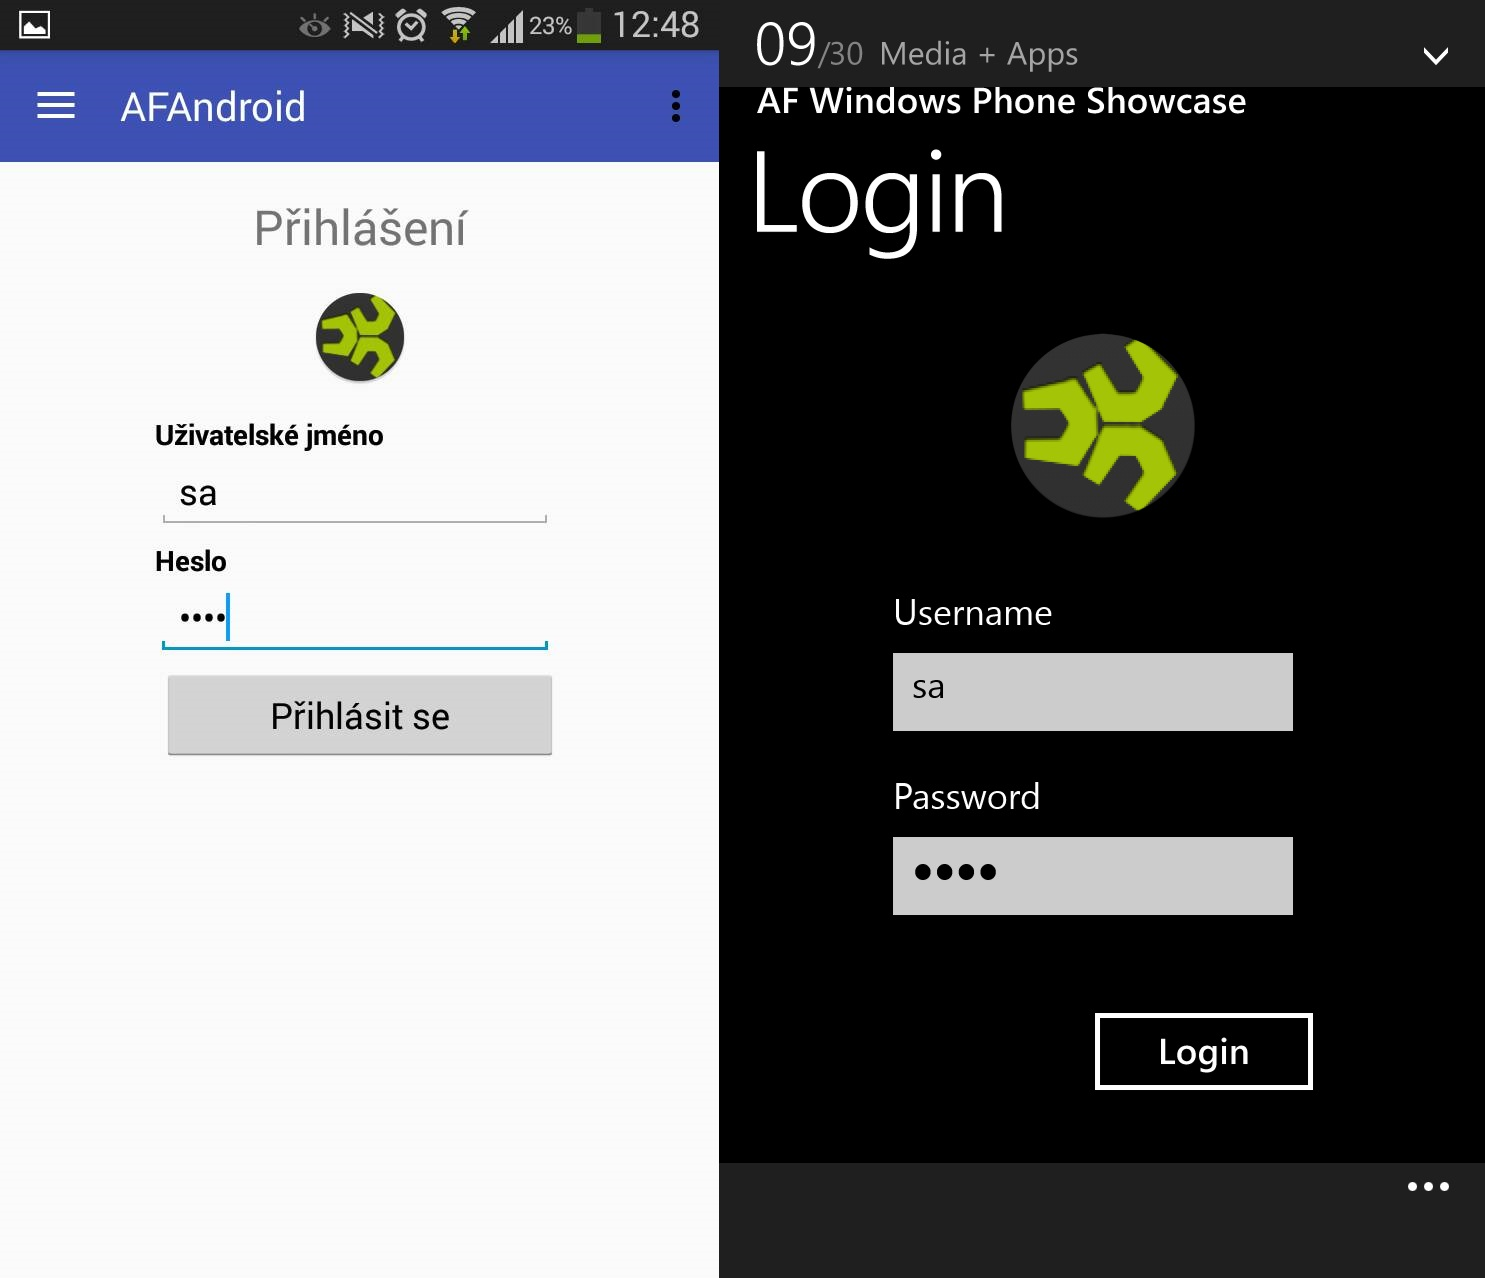
\includegraphics[width=0.5\linewidth]{figures/screenshots/Login}
\caption{Ukázkové projekty - přihlášení}  
\label{img:login}
\end{figure}

\subsection{Správa zemí}
Tato sekce obsahuje list, který zobrazuje již existující země a formulář, kterým země lze vytvořit nebo upravit, což reprezentuje obrázek \ref{img:country}. Pro upravení existující země stačí na zemi kliknout a zobrazí se její náhled ve formuláři níže. Pokud je takto formulář naplněn, tak jeho změna zemi ve formuláři edituje, pokud je formulář prázdný je provedením změn vytvořena země nová. Upravovat a přidávat země smí jen admin, obyčejný uživatel má prvky formuláře neaktivní. V případě, že by došlo k chybě a obyčejný uživatel by přesto poslal data na server, kontroluje se uživatelská role i na serveru. Po přidání či úpravě země se uživateli zobrazí výsledek akce v Androidu formou Toast zprávy, ve WP formou dialogu. Obrazovka disponuje také tlačítky na resetovaní a vyčištění formuláře.
\subsection{Správa absencí}
Dalším případem, kdy zavisí na uživatelské roli je obrazovka reprezentující správu absencí. V této sekci je pro zobrazení absencí vytvořen list a pod ním je umístěn formulář, do kterého lze nahrát data z listu a případně je upravit. Každá uživatelská role vidí v listu různá data, obyčejný uživatel vidí pouze své vytvořené absence a má možnost je zrušit či nechat ve stavu, kdy žádá o schválení, což je zobrazeno na obrázku \ref{img:AbsenceManagement}. Adminstrátor vidí všechny absence včetně svých a může je schvalovat, rušit nebo zamítnout, což je patrné z obrázku \ref{img:AbsenceManagementAdmin} . V případě, že admin žádost schválí nebo zamítne, mizí běžnému uživateli absence z listu a již s ní nelze operovat, administrátor vidí absence ve všechy čtyřech stavech. 
\subsection{Správa absenčních typů}
Každá země má své typy absencí, které lze použít. Uživatel má na výběr z typů absencí, které přísluší zemi, která je uživateli nastavena. Data v listu, který je na obrazovce se správou typů, jsou závislé na volbě země, která je reprezentována formulářem o jednom prvku, ze kterého se předá pro tvorbu listu identifikátor vybrané země. Tento formulář je v Android aplikaci ve vrchní části obrazovky. Ve Windows Phone verzi byl zvolen jiný přístup, při pokusu přejít na tuto obrazovku je nejprve zobrazen dialog s formulářem, pro výběr země. Po vybrání země a potvrzení se zobrazí již příslušný list. Formulář, který je v Android aplikaci pod listem je ve WP verzi na vedlejší stránce. Při kliku na položku v listu aplikace přejde sama na vedlejší stránku s naplněných formulářem, při úspěšném přidání či úpravě přejde aplikace z formuláře zpět na list. Tento přístup byl zvolen pro demostraci toho, že vytvořené komponenty lze opravdu vložit do jakéhokoliv jiného prvku uživatelského rozhraní. Příslušná část aplikace je zobrazena na obrázku \ref{img:AbsenceType}.
\subsection{Uživatelský profil}
Každý uživatel má svůj profil, který může v aplikaci upravovat. Tato obrazovka slouží hlavně k demostraci většiny typů aktivních prvků, které umí framework interpretovat. Pole ve formuláři upravující profil také podléhají validacím. Obrázek \ref{img:profileValidations} zobrazuje dvě z nich, validaci pravidel REQUIRED a MAX z tabulky \ref{table:validations}. Také je patrné, že je Android aplikace převážně v češtině a WP verze v angličtině, za což je zodpovědná lokalizační část frameworku. Ne všechny popisky však ze serveru přichází ve formě klíčů k přeložení a nejsou proto lokalizovány. 

\chapter{Závěr}
\section{Budoucí vývoj}
Testování s uživateli dopadlo dobře a na základě toho bychom chtěli framework dále rozvíjet. Serverová část frameworku umožňuje vytvářet definice komponent. Tyto informace lze využít ke stavbě komponent na libovolné platformě. V další iteraci, bychom rádi přidali možnost využívat tyto definice na mobilní platformě a v dynamicky se rozvíjejícím frameworku AngularJS. S tím se bude pojit vyjmutí specifických modulů z části AFSwinx a jejich propagace do jiného projektu, který pak bude využit na těchto platformách. Z hlediska bezpečnosti lze zatím využít autorizace typu basic, v tomto ohledu bychom rádi projekt rozšířili o další možnosti například o oAuth. Framework nyní podporuje množinu validací, kterou budeme dále rozšiřovat. Budou provedeny další UX testy, na základě kterých může být upraven způsob, jakým framework funguje.

Iterace a rozvoj frameworku by měl vyústit v plně nasaditelnou technologii, kterou bychom chtěli distribuovat v rámci AspectFaces. Tím docílíme toho, že vývojář při využití tohoto projektu definuje definice pouze jednou a klienti je budou moci používat na různých platformách. Výhodou bude velmi rychlé prototypování a vytváření aktivních prvků, které~budou reflektovat změny v serverové konfiguraci a změny v modelu, který reprezentují.
\section{Zhodnocení práce}
Cílem práce bylo navrhnout způsob, jakým lze aspektově generovat uživatelská rozhraní na~platformě Java~SE. Práce se zaměřuje především na tlusté klienty k serverovým aplikacím. Framework byl navržen, sestaven a otestován pomocí ukázkové aplikace. Použitelnost frameworku byla testována při testech použitelnosti s cílovou skupinou uživatelů.

Nejprve bylo potřeba zpracovat již existující řešení a zhodnotit jejich výhody a nevýhody. Již v této fázi bylo zřejmé, že pokud budou objekty dat centralizovány, bude zjednodušena jejich správa a možné úpravy. Způsob má i jednu nevýhodu, pokud si klient od serveru vyžádá data, potom je struktura, kterou obdrží, závislá na datech. V případě že se mění struktura dat, musí se přizpůsobovat i klient. Tuto nevýhodu lze odstranit dynamickou inspekcí dat, která vytvoří definice, jež se využijí k sestavení komponenty a poté ji nastaví na základě obdržených dat. Toto nastavení je dynamické. Klient se tedy nemusí přizpůsobovat, pokud server změní strukturu dat, neboť mu tuto skutečnost server sdělí ihned při generování definic.

Byl vytvořen návrh definic dat, pomocí kterých umí klient vytvořit formuláře a tabulky. Tyto definice jsou generovány na serverové straně s využitím frameworku AspectFaces a poté odeslány na klienta, kde jsou interpretovány. Klient umí na základě těchto definic vytvářet tabulky či formuláře, které sestaví podle určeného layoutu a nastaví všem aktivním prvkům validátory. Při obdržení dat umí tyto data správně vložit do komponent a následně datový objekt znovu sestavit pouze ze znalosti definice. Klientská strana předem nezná objekt, jenž obdrží a může tedy pružně reagovat na změny datových definic. Z hlediska bezpečnosti podporuje klient komunikaci pomocí HTTPS a autorizaci typu basic. Framework, je tedy rozdělen na klientskou a serverovou část, s tím, že klientovi stačí vložení závislosti na~klientskou stranu a serveru na serverovou stranu a v případě využití AspectFaces i závislost na~tento projekt. Ke generování dat se využívá knihovna třetí strany. Výhodou je její stabilnost a~fakt, že disponuje velkou škálou možností, jak uživatelské rozhraní generovat. Framework zohledňuje uživatelské role a nabízí anotace, které lze využít při generování. Šablony byly upraveny tak, aby vytvářely jednotnou definici použitelnou na více platformách. Definice je tedy platformě nezávislá. 

Při vývoji frameworku jsem se musel na problém zaměřit jak z hlediska funkčnosti, tak z hlediska použitelnosti, a zohlednit budoucí vývoj frameworku. Bylo potřeba navrhnout způsob, jakým se bude model generovat a následně přenášet do klientské části aplikace. V~klientské části bylo třeba model zpracovat a na jeho základě sestavit konkrétní komponenty, se kterými může klient dále pracovat, a ve kterých bude zohledněna bezpečnost, layout a~vnitřní reprezentace dat. Tyto vlastnosti byly v analytické části rozpracovány a~v~implementační části vytvořeny. Výsledný framework byl otestován s uživateli při testech použitelnosti, ve kterých jsem se zaměřil na způsob, jakým uživatelé framework využívají. Některé části pokrývají unit testy a také byla vytvořena ukázková serverová a klientská aplikace. Tato ukázková aplikace sloužila k alfa testování a do budoucnosti bude sloužit pro smoke testy. Framework byl úspěšně navržen, vytvořen a otestován.

%*****************************************************************************
% Seznam literatury je v samostatnem souboru reference.bib. Ten
% upravte dle vlastnich potreb, potom zpracujte (a do textu
% zapracujte) pomoci prikazu bibtex a nasledne pdflatex (nebo
% latex). Druhy z nich alespon 2x, aby se poresily odkazy.

% originally following specification for bibliography formating was used
%\bibliographystyle{abbrv}

% Here is an improvment by Petr Dlouhy (April 2010).
% It is mainly for supervisors who expect Czech fomrating rules for references
% Additional feature is live url addresses to sources from your pdf file
% It requires the file csplainnat.bst (included in this sample zipfile).
\bibliographystyle{csplainnat}

%bibliographystyle{plain}
%\bibliographystyle{psc}
{
%JZ: 11.12.2008 Kdo chce mit v techto ukazkovych odkazech take odkaz na CSTeX:
\def\CS{$\cal C\kern-0.1667em\lower.5ex\hbox{$\cal S$}\kern-0.075em $}
\bibliography{reference}
}

\appendix
\chapter{Seznam použitých zkratek}

\begin{description}
\item[A7B36ASS] Architektury softwarových systémů
\item[GNU GPL] GNU General Public License
\item[OCL] Object Constraint Language
\item[UML] Unified Modeling Language
\item[MVC] Model-view-controller
\item[AJAX] Asynchronous JavaScript and XML
\item[JAAS] Java Authentication and Authorization Service
\item[SSH] Secure Shell
\item[REST] Representational State Transfer
\item[JDBC] Java Database Connectivity
\item[OSGI] Open Services Gateway Initiative
\item[HTTP] Hypertext Transfer Protocol
\item[ORM] Object relational mapping
\item[EJB] Enterprise JavaBean
\item[JPA] Java Persistence API
\item[API] Application programming interface

\end{description}

%*****************************************************************************
\chapter{Instalační a uživatelská příručka}
Framework byl vytvořen jako Maven projekt, jeho přidání do již existující aplikace lze buďto jako knihovnu nebo jako Maven závislost. Způsob jakým lze integrovat projekt a jak ho používat je detailně popsán v uživatelské příručce na přiloženém CD. 
\section{Maven závislosti}
Nejprve je potřeba provést build frameworku. Zdrojové kódy jsou na přiloženém CD. Framework zatím není v žádném z veřejně dostupných repositářích. Poté lze na serveru stranu přidat následující závislosti:
\begin{lstlisting}[caption={Závislosti na serveru},
label={code:mavenDependency}, basicstyle=\footnotesize]
<dependency>
	<groupId>com.tomscz.af</groupId>
	<artifactId>AFRest</artifactId>
	<version>0.0.1-SNAPSHOT</version>
</dependency>
<dependency>
	<groupId>com.codingcrayons.aspectfaces</groupId>
	<artifactId>javaee-connector</artifactId>
	<version>1.5.0-SNAPSHOT</version>
</dependency>
<dependency>
	<groupId>com.codingcrayons.aspectfaces</groupId>
	<artifactId>annotation-descriptors</artifactId>
	<version>1.5.0-SNAPSHOT</version>
</dependency>
\end{lstlisting}
Repozitář pro aspectFaces je zde:
\begin{lstlisting}[caption={AspectFaces repozitář },
label={code:mavenAspectFacesRepo}]
<repository>
	<id>codingcrayons-repository</id>
	<name>CodingCrayons Maven Repository</name>
	<url>http://maven.codingcrayons.com/content/groups/public/</url>
</repository>
\end{lstlisting}
Do složky WEB-INF je potřeba rozbalit soubor templates.zip, v kterém je předpřipravená konfigurace a do web.xml je potřeba přidat listener, který provede nastavení AspectFaces během startu. 
\begin{lstlisting}[caption={AspectFaces listener},
label={code:mavenAspectFacesBootStrap}, basicstyle=\footnotesize]
<listener>
	<!-- Include Aspect Faces listener to perform proper framework initialization 
	during application start -->
	<listener-class>com.codingcrayons.aspectfaces.plugins.j2ee.AspectFacesListener</listener-class>
</listener>
\end{lstlisting}
Na klientskou stranu je potřeba přidat následující závislost:
\begin{lstlisting}[caption={Závislost na klientské straně},
label={code:mavenAFSwinx}, basicstyle=\footnotesize]
<dependency>
	<groupId>com.tomscz.af</groupId>
	<artifactId>AFSwinx</artifactId>
	<version>0.0.1-SNAPSHOT</version>
</dependency>
\end{lstlisting}
\section{Ukázkový projekt}
Ukázkový projekt se svojí klientskou a serverovou částí jsou již vytvořeny a přiloženy na CD. Serverovou část lze bez dodatečné konfigurace spusti na serveru GlassFish V3. Ukázkový projekt je možné spustit i na GlassFish V4 nicméně, při deployi aplikace je v konzoli zobrazena chyba, avšak aplikace je plně funkční. Na toto chování byl založen bug, který není prozatím vyřešen. Je potřeba provést následující:
\begin{enumerate}
\item Rozbalte aplikační server GlassFish, který je přiložen na CD nebo si stáhněte verzi 3 z http://www.oracle.com/technetwork/middleware/glassfish/downloads/java-archive-downloads-glassfish-419424.html Verzi 4 lze stáhnout z http://dlc.sun.com.edgesuite.net/glassfish/4.1/release/glassfish-4.1.zip
\item Rozbalte soubor, ve složce bin spoustě utilitu asadmin napsáním asadmin
\item Vložte následující příkaz: start-domain domain1
\item Vložte následující příkaz deploy PATHTOFILE/AFServer.war
\item Otevřete webový prohlížeč na adrese http://localhost:8080/AFServer - zobrazí se text: I am alive. Serverová strana nedisponuje grafickým uživatelským rozhraním. Funkčnost můžete otestovat pomocí rest klienta například na adrese http://localhost:8080/AFServer/rest/country/list - content-type: application/json metoda GET.
\end{enumerate}
Nyní je potřeba spustit klientskou část aplikace. Ve složce s Showcase.jar, který je přiložen na CD spusťte java -jar Showcase.jar . Aplikace bude spuštěna.





\chapter{UML diagramy}
V této sekci naleznete použité UML diagramy, na které bylo v textu odkazováno.
\begin{figure}
\begin{center}
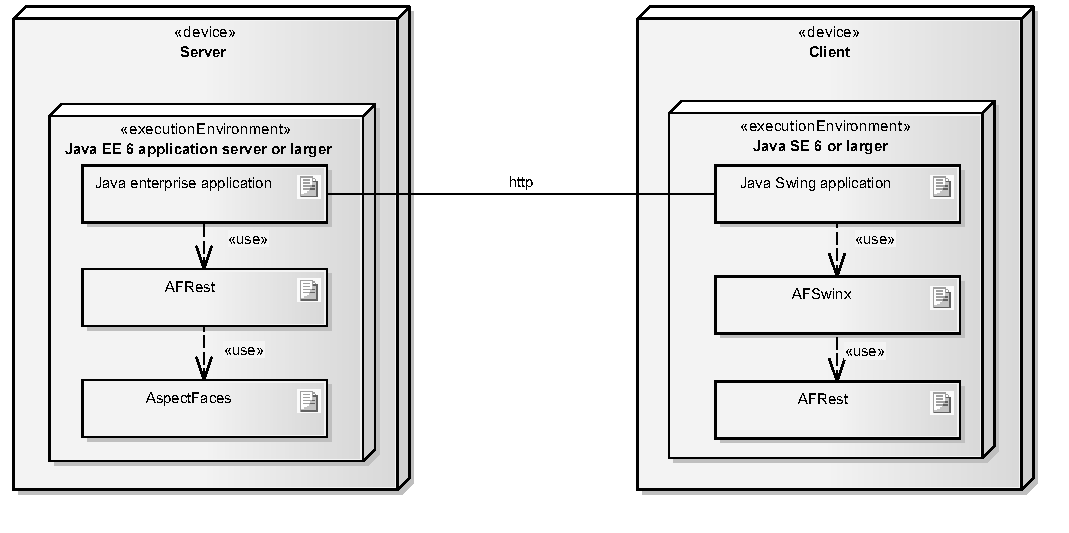
\includegraphics[angle=270]{images/deploymentDiagram}
\caption{Diagram nasazení}
\label{img:deploymentDiagram}
\end{center}
\end{figure}

\begin{figure}
\begin{center}
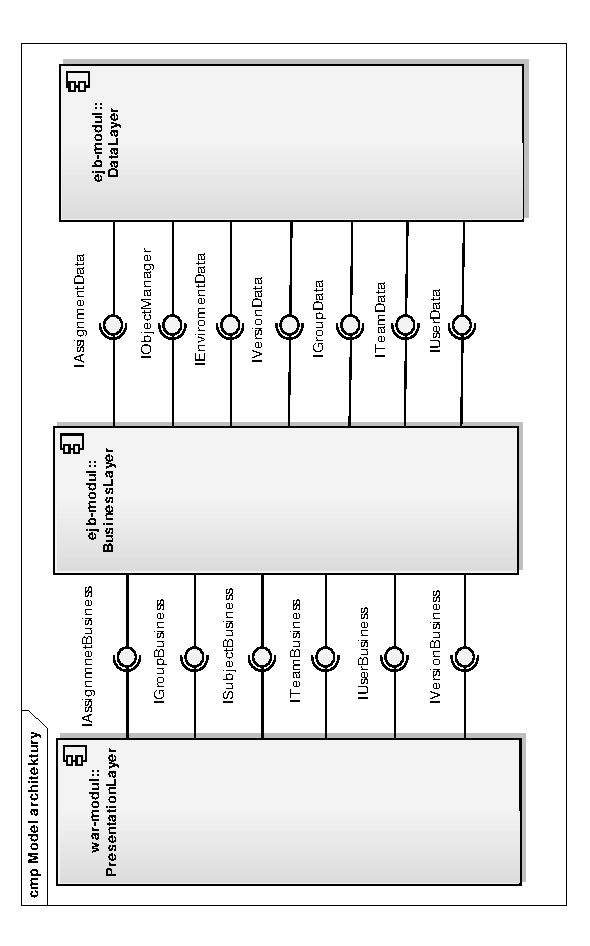
\includegraphics[angle=270]{images/architektura}
\caption{Architektura aplikace}
\label{img:architektura}
\end{center}
\end{figure}



\begin{figure}[h!]
\begin{center}
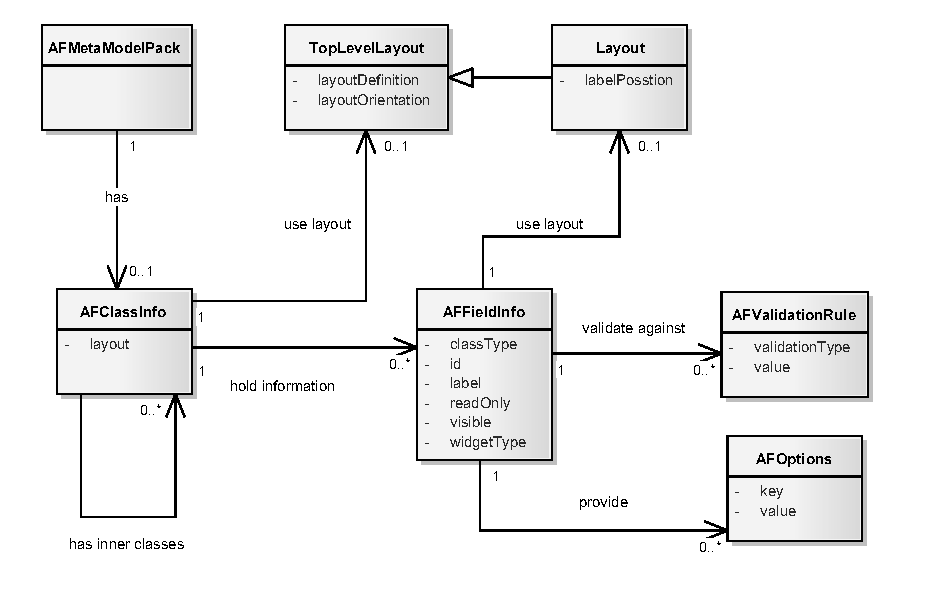
\includegraphics[width=\linewidth]{images/domainModel}
\caption{Doménový model systému pro zadávání a odevzdávání úkolů}
\label{img:domainModel}
\end{center}
\end{figure}

\begin{figure}
\begin{center}
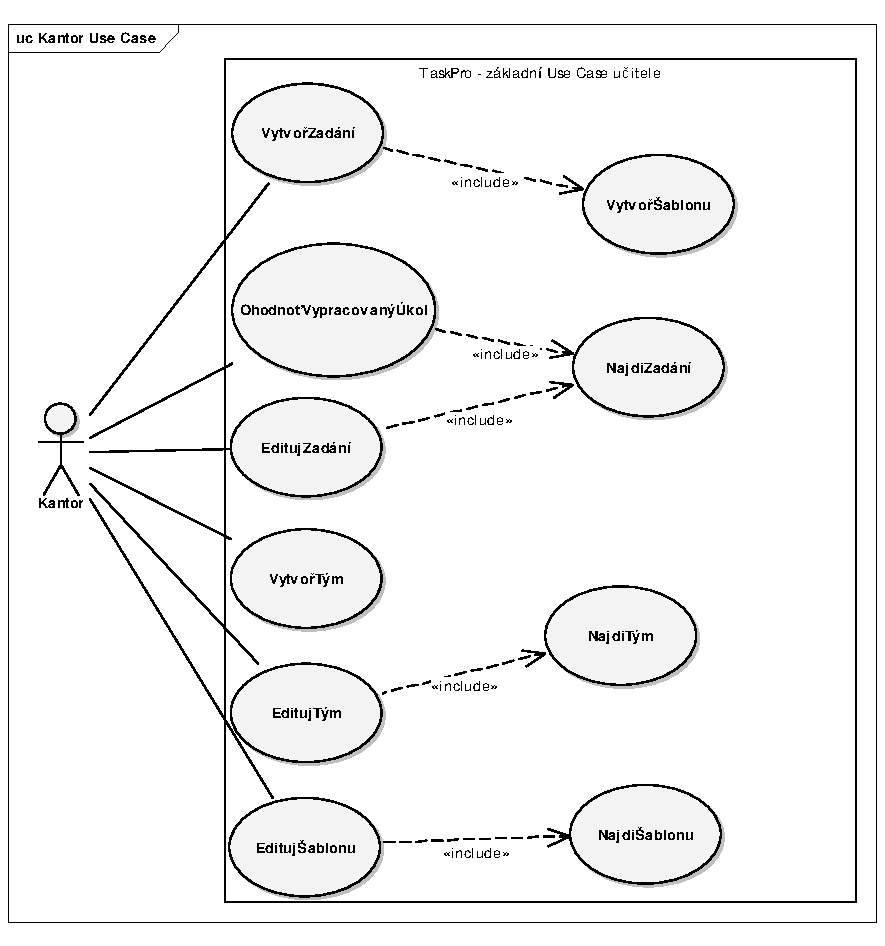
\includegraphics{images/kantorUseCase}
\caption{Základní případy užití pro učitele}
\label{img:kantorUseCase}
\end{center}
\end{figure}

\begin{figure}
\begin{center}
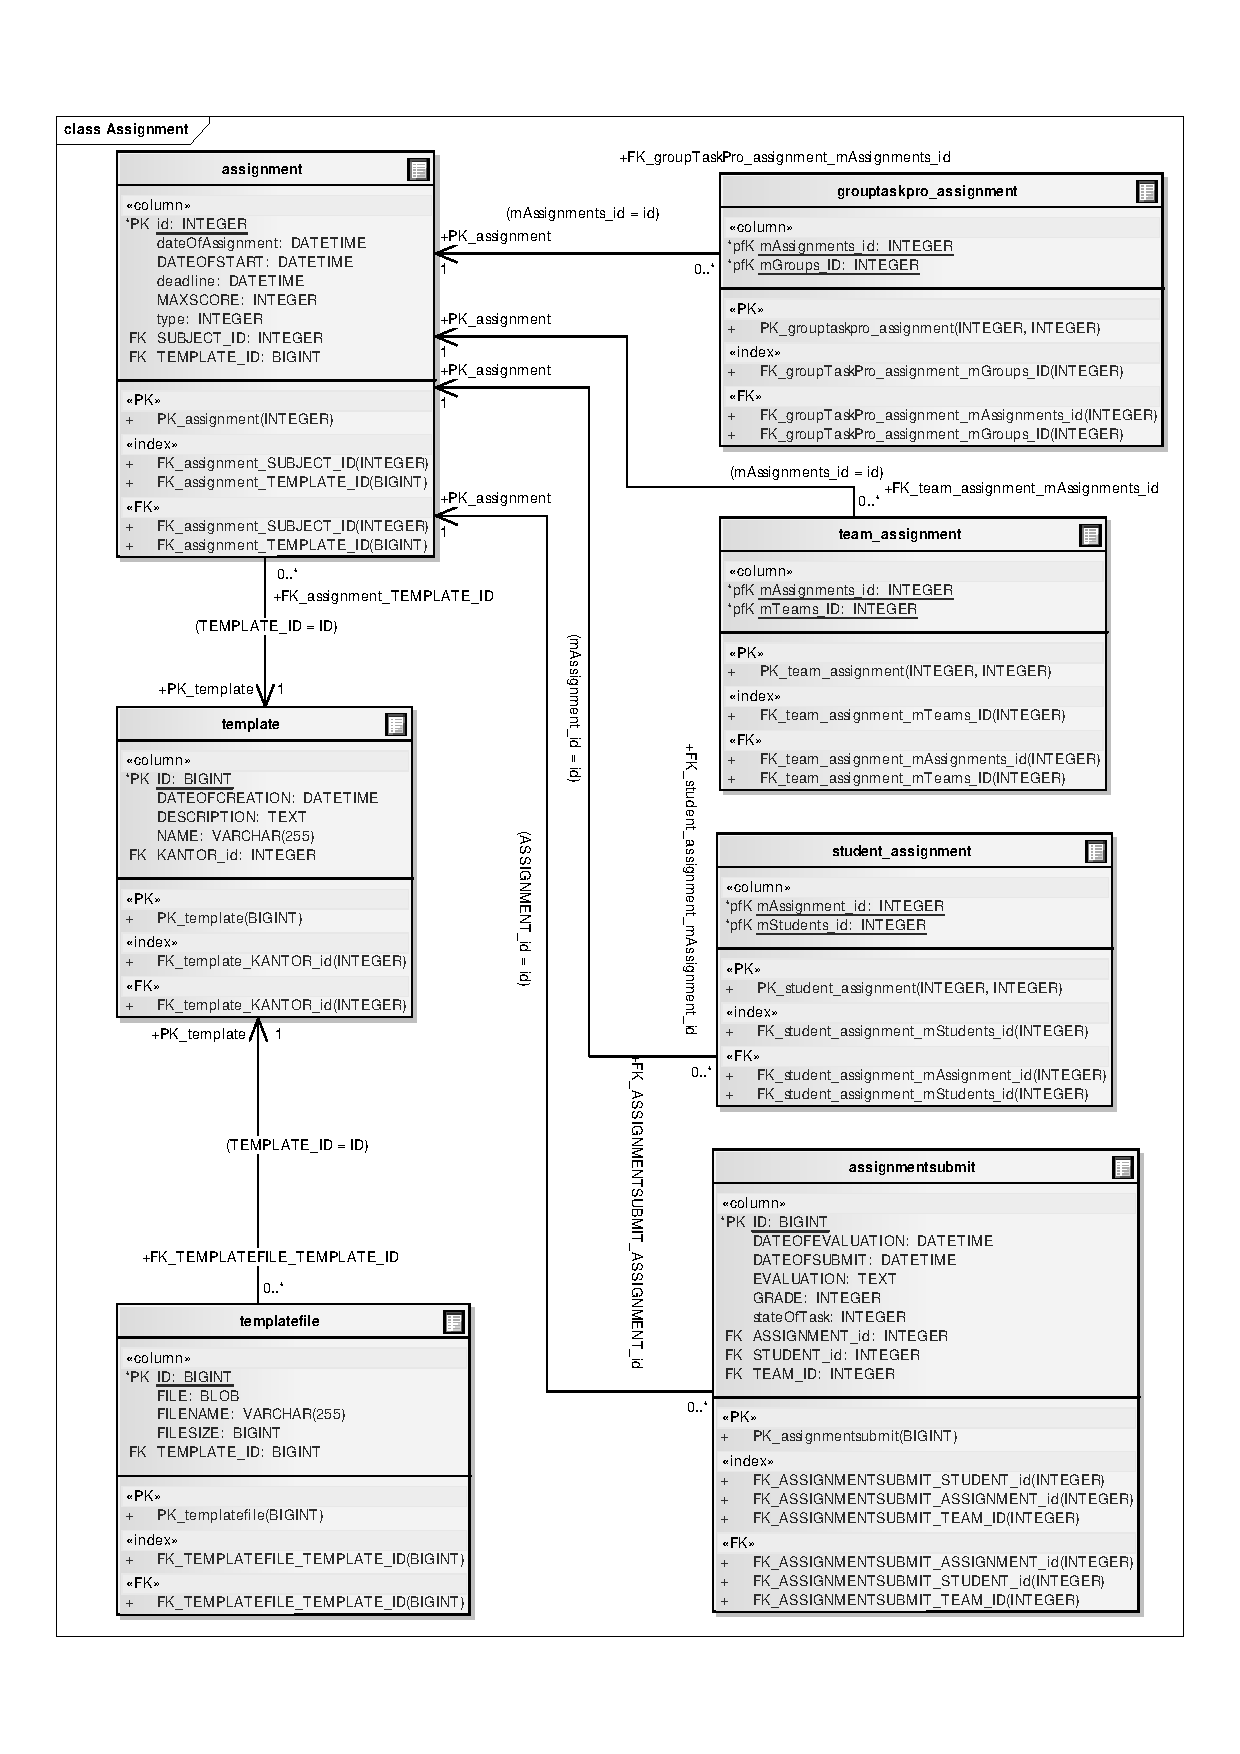
\includegraphics[width=\linewidth]{images/assignmentRelation}
\caption{Relační schéma zadání}
\label{img:assignmetnRelation}
\end{center}
\end{figure}

\begin{figure}
\begin{center}
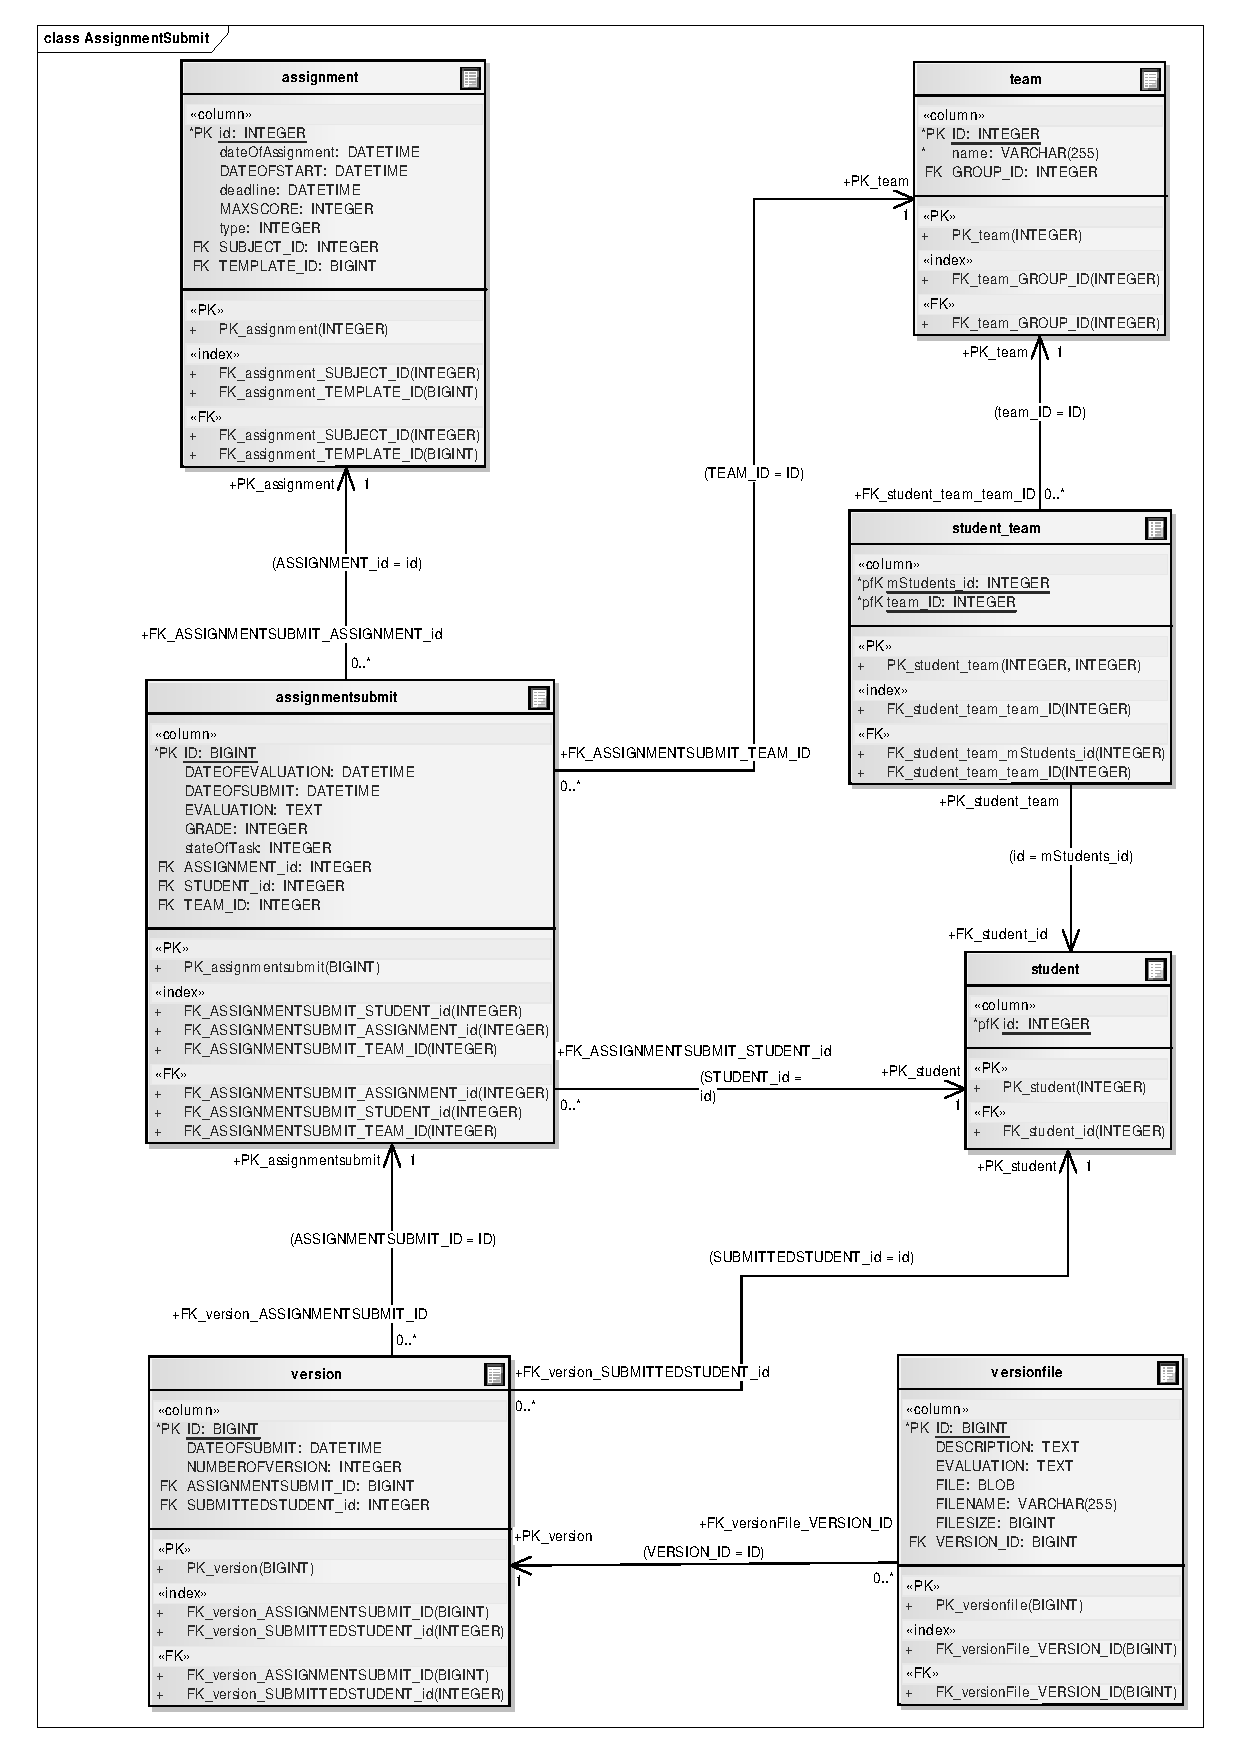
\includegraphics[width=\linewidth]{images/assignmentSubmitRelational}
\caption{Relační schéma odevzdání zadání}
\label{img:assignmnetSubmitRelation}
\end{center}
\end{figure}	

\begin{figure}
\begin{center}
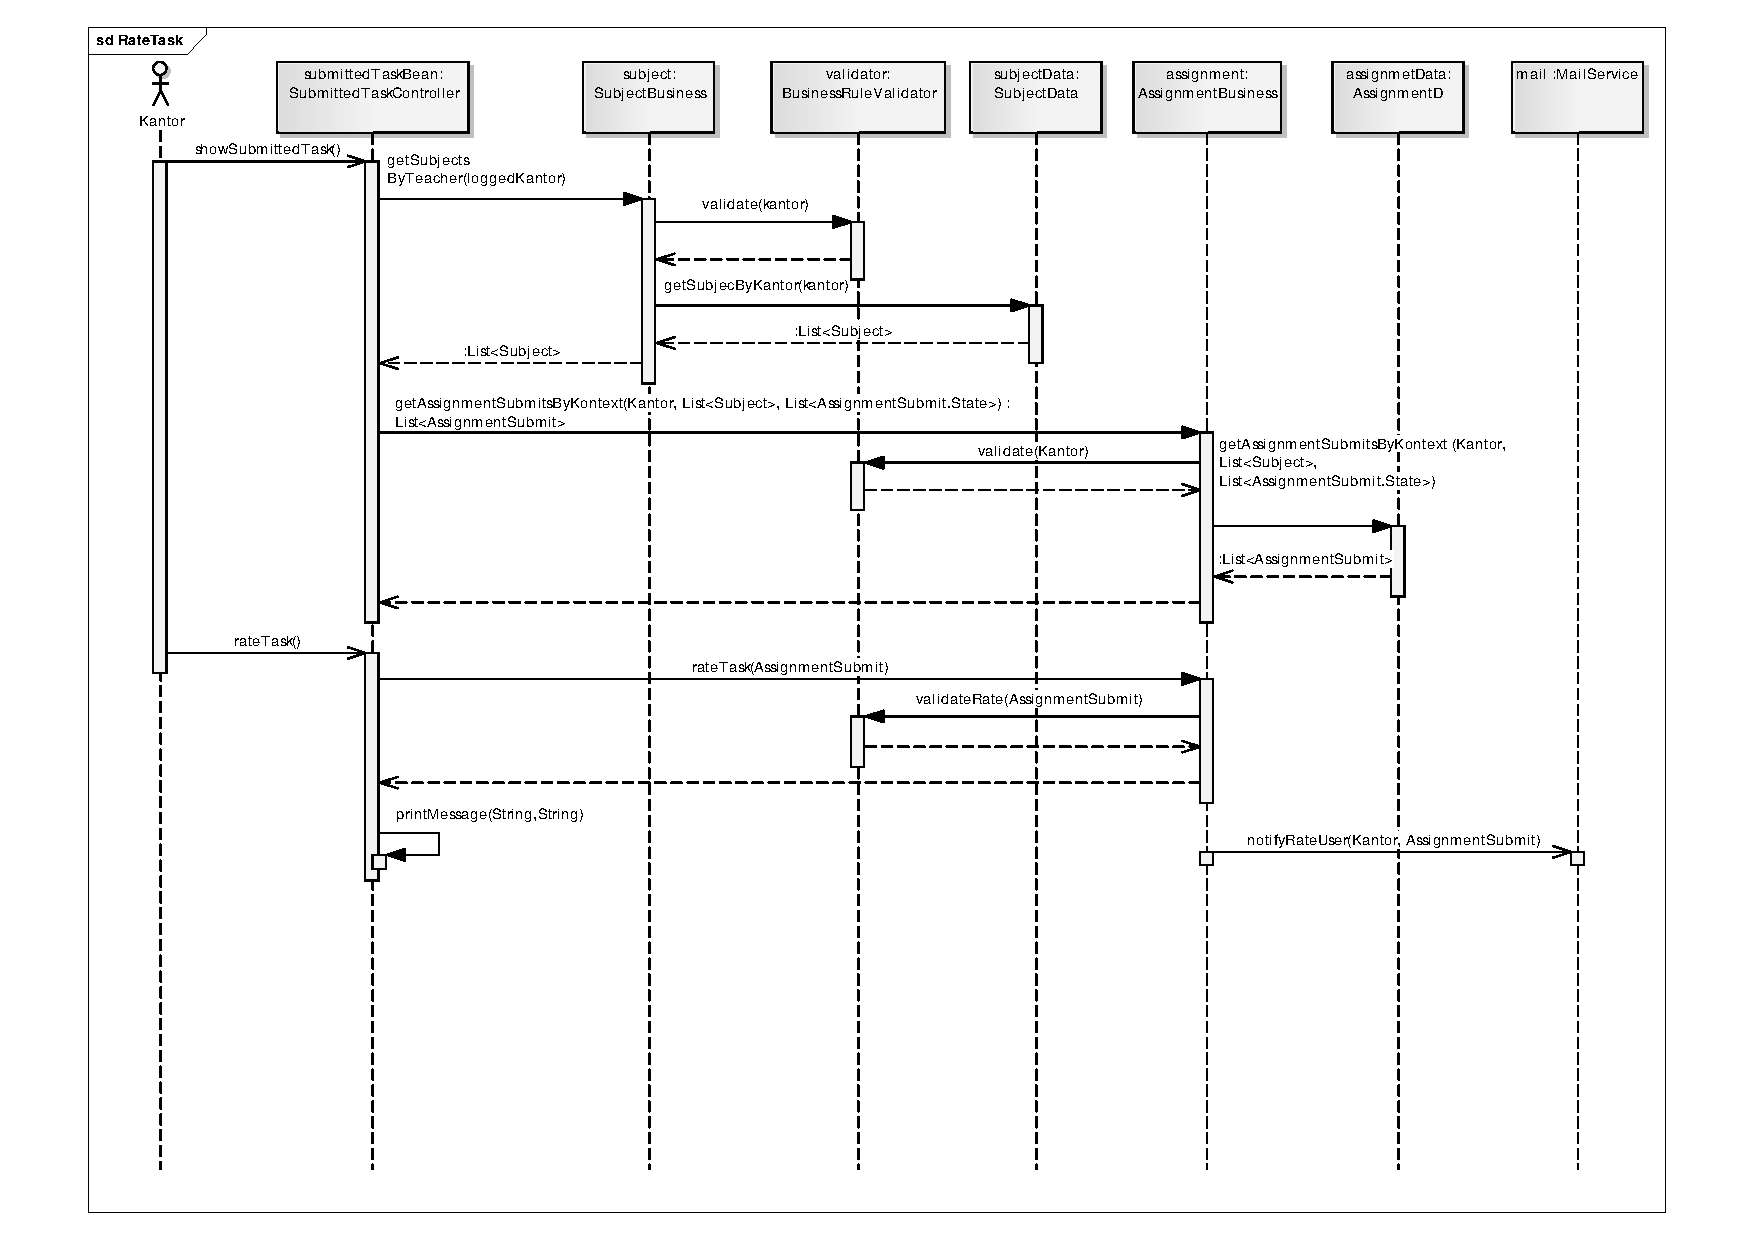
\includegraphics[width=\linewidth]{images/sdRate}
\caption{Systémový sekvenční diagram zachycující oznámkování úkolu}  
\label{img:ssdRate}
\end{center}
\end{figure}

%*****************************************************************************

%*****************************************************************************
\chapter{Obsah přiloženého CD}

\begin{figure}[h!]
\begin{center}
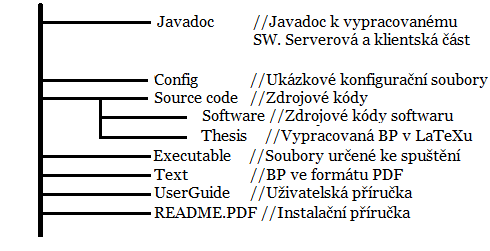
\includegraphics{images/cdContent}
\caption{Obsah přiloženého CD}  
\label{img:cd}
\end{center}
\end{figure}
\end{document}
